% Template LaTeX Tesis Ciencia de la Computación UCSP
% 2022

\documentclass[a4paper,openany,12pt]{book}
\usepackage[utf8]{inputenc}
\usepackage{graphicx}
\usepackage[spanish,mexico]{babel}
\usepackage{sty/fancyhdr}
\usepackage{ae}
\usepackage[left=2.5cm,right=2.5cm,top=3cm,bottom=2cm]{geometry}
\usepackage[printonlyused]{acronym}
\usepackage{xspace}
\usepackage{sty/hlundef}
\usepackage{sty/tesis}
\usepackage{setspace}
\usepackage{booktabs}

\title{** Título de la Tesis **}
\title{Arquitectura de razonamiento estructural basada en representación intermedia para la mitigación de alucinaciones en la generación de consultas empresariales sobre el estándar híbrido SQL/PGQ}

\author{Guido Luis Tapia Oré}


\advisor{Dra. Regina Paola Ticona Herrera}


\date{** Arequipa, Julio 2026 **}

%\examinerone{Prof. Dr. Hidalgo Buena Gente}{Presidente}%
%\examinertwo{Prof. Dr. Antero A. Gal Oppe}{Secretario}%
%\examinerthree{Prof. Dr. Liu Xiao Ling}{University of ...} % of being the case

\dedicado{A mi familia por su incondicional apoyo en este proceso, a los profesores que fueron una guía en este proceso de investigación, a mis compañeros que ayudaron a no rendirme en este proceso.}

\begin{document}
\pagestyle{fancy}

\maketitle %Compone la carátula y la dedicatoria
\newpage

%\approved{\tres}%  {\tres} or {\cuatro}

%mayores detalles de como usas las abreviaturas (acronimos)
% vea: http://www.ctan.org/tex-archive/macros/latex/contrib/acronym/
% hay un manual en pdf en esa misma direccion

\chapter*{Abreviaturas}

\begin{acronym}
\acro{API}{Application Programming Interface}
\acro{AST}{Abstract Syntax Tree}
\acro{IA}{Inteligencia Artificial}
\acro{LLM}{Large Language Model}
\acro{NL}{Natural Language}
\acro{NL2SQL}{Natural Language to SQL}
\acro{NLP}{Natural Language Processing}
\acro{PGQ}{Property Graph Queries}
\acro{RAG}{Retrieval-Augmented Generation}
\acro{RDBMS}{Relational Database Management System}
\acro{RI}{Representación Intermedia}
\acro{SOTA}{State of the Art}
\acro{SQL}{Structured Query Language}
\acro{SQL/PGQ}{SQL Property Graph Queries}
\end{acronym}


\input{Agradecimientos} %Inserta los agradecimientos
\begin{resumen}
La generación automática de consultas a bases de datos a partir de lenguaje natural (\emph{text-to-query}) ha avanzado de la mano de los modelos extensos de lenguaje, pero en entornos empresariales aún produce fallas sistemáticas de fidelidad estructural: referencias a tablas o columnas inexistentes, uniones inválidas y patrones de grafo incoherentes con el esquema. El problema se intensifica bajo el estándar híbrido \ac{SQL}/\ac{PGQ} (ISO/IEC 9075-16:2023), donde la generación debe operar simultáneamente sobre un esquema relacional y un grafo de propiedad declarado sobre este.

Esta tesis propone una arquitectura de razonamiento estructural basada en una representación intermedia tipada, IR-SQL/PGQ, que media entre la salida del modelo de lenguaje y la consulta ejecutable. La arquitectura articula cuatro componentes: un anclaje al esquema dual que reduce el espacio de búsqueda; la representación intermedia, expresable de forma uniforme sobre los regímenes relacional, de grafo e híbrido y decidible mediante reglas locales de tipado; un compilador determinista hacia \ac{SQL}/\ac{PGQ}; y un bucle de verificación en cascada que opera sobre la propia representación intermedia con retroalimentación estructurada por descriptores categóricos.

La validación experimental se desarrollará sobre los \emph{benchmarks} Spider y BIRD para el régimen relacional y sobre un corpus propio para el régimen híbrido \ac{SQL}/\ac{PGQ}. Las métricas reportadas incluirán corrección, tasa de alucinación, transferibilidad a entornos heterogéneos y coste agregado por consulta. La hipótesis central, sujeta a verificación empírica, es que la mediación por representación intermedia tipada con verificación en cascada reduce las alucinaciones referenciales y estructurales respecto a la generación directa, sin comprometer el coste sostenido en escenarios empresariales.
\end{resumen}
 %Inserta el resumen
\begin{abstract}
Automatic text-to-query generation has progressed alongside large language models, yet in enterprise settings it still exhibits systematic failures in structural fidelity: references to non-existent tables or columns, invalid joins, and graph patterns inconsistent with the schema. These failures intensify under the hybrid \ac{SQL}/\ac{PGQ} standard (ISO/IEC 9075-16:2023), where generation must operate simultaneously over a relational schema and a property graph defined on top of it.

This thesis proposes a structural reasoning architecture based on a typed intermediate representation, IR-SQL/PGQ, that mediates between the language model's output and the executable query. The architecture articulates four components: a dual-schema grounding stage that narrows the search space; the intermediate representation itself, uniformly expressive over the relational, graph, and hybrid regimes and decidable through local typing rules; a deterministic compiler to \ac{SQL}/\ac{PGQ}; and a cascaded verification loop that operates on the intermediate representation with structured feedback through categorical descriptors.

Empirical validation will be conducted on the Spider and BIRD benchmarks for the relational regime and on a purpose-built corpus for the hybrid \ac{SQL}/\ac{PGQ} regime. Reported metrics will include correctness, hallucination rate, transferability across heterogeneous environments, and aggregated per-query cost. The central hypothesis, subject to empirical verification, is that mediation through a typed intermediate representation with cascaded verification reduces referential and structural hallucinations relative to direct generation, without compromising sustained cost in enterprise scenarios.
\end{abstract}
 %Inserta el abstract

\pagenumbering{roman}
\setcounter{page}{1}
\pagestyle{plain}

\tableofcontents %Inserta el índice general
\listoftables %Inserta el índice de cuadros
\listoffigures %Inserta el índice de figuras

%%%%%%%%%%%%%%%%%%%%%%%%%%%%%%%%%%%%%%%%%%%%%%%%%%%%%%%%%%%%%%%%%%%%%
%%%%   En esta parte deberas incluir los archivos de tu tesis   %%%%%
%%%%%%%%%%%%%%%%%%%%%%%%%%%%%%%%%%%%%%%%%%%%%%%%%%%%%%%%%%%%%%%%%%%%%

\pagestyle{plain}
\pagenumbering{arabic}
\setcounter{page}{1}
\chapter{Introducción}
\label{chap:introduction}

Este capítulo establece el contexto, la motivación y el problema de investigación que aborda la presente tesis, cuyo enfoque central radica en el diseño de una arquitectura de razonamiento estructural, basada en \ac{RI}, para mitigar las alucinaciones en la generación \emph{text-to-query} de consultas empresariales complejas, específicamente orientada al estándar híbrido \ac{SQL}/\ac{PGQ}.

Esta investigación se sitúa en la intersección entre los \acp{LLM}, los sistemas de gestión de bases de datos relacionales (\acp{RDBMS}) y los lenguajes de consulta híbridos, pues estos lenguajes combinan el paradigma relacional tradicional con las consultas sobre grafos de propiedades (\emph{property graphs}), un modelo recientemente formalizado en estándares internacionales como ISO/IEC \cite{ISO9075_16_2023}.

Como se evidenciará en el posterior desarrollo, el diseño propuesto representa una respuesta estructurada al creciente interés de la industria por desplegar interfaces en lenguaje natural altamente fiables en entornos empresariales a gran escala. Reducir las alucinaciones y mantener la consistencia lógica constituyen retos críticos actuales \cite{WrenAI2025, TA-SQL2024}, los cuales demandan métodos avanzados que integren el razonamiento tabular y de grafos \cite{STRuCT-LLM2026}.


%A pesar de que la generación text-to-queries (Text→Query) con modelos de lenguaje grandes \ac{LLM} se ha desarrollado rápidamente, en situaciones empresariales todavía presenta fallas sistemáticas en términos de seguridad operacional, fidelidad al esquema y corrección semántica. Estas fallas se presentan en forma de alucinaciones específicas de consulta: referencias a columnas/tablas/atributos que no existen, rutas de uniones inventadas, errores en las agregaciones y malentendidos en las condiciones. En el caso de los grafos, son patrones o etiquetas de recorrido que no concuerdan con el modelo gráfico. Investigaciones actuales sobre evaluación "realista" indican que el desempeño en benchmarks tradicionales no se refleja correctamente en los flujos empresariales: 

\section{Motivación y Contexto}
\label{sec:motivacion_contexto}

En el contexto actual de la adopción de \acp{LLM} en procesos empresariales y el creciente interés por integrarlos en la optimización de flujos de trabajo, se evidencia una clara tendencia hacia interfaces basadas en lenguaje natural \cite{Data2Decisions}, en detrimento de las interfaces gráficas tradicionales. Este cambio es particularmente notable en organizaciones \emph{data-driven}, cuya toma de decisiones depende de la capacidad de responder preguntas de negocio en ciclos cortos y con altas garantías de calidad \cite{llm-insight}. En este marco, las interfaces en lenguaje natural para la consulta de datos han resurgido con fuerza, habilitando experiencias de \emph{self-service analytics}. Estas permiten que perfiles no técnicos formulen preguntas en texto libre y lenguaje cotidiano, obteniendo resultados estructurados sin la necesidad de escribir manualmente consultas complejas \cite{NLinterfaces}. 

Sin embargo, el despliegue de estos modelos en entornos de producción demanda el cumplimiento de tres pilares críticos: (i) \emph{integridad técnica}, que garantiza tanto la ejecutabilidad en el \ac{RDBMS} como la fidelidad semántica de la consulta \cite{spider2_2025}; (ii) \emph{seguridad y gobernanza}, mediante mecanismos de control de acceso basado en roles (RBAC) y auditoría para prevenir la exfiltración de datos sensibles \cite{SAFENLIDB}; y (iii) \emph{robustez y escalabilidad del esquema}, asegurando que el modelo mantenga su precisión frente a catálogos de datos masivos, dinámicos y con nomenclaturas complejas \cite{llmfk}.


Asimismo, a pesar de los avances acelerados, los \acp{LLM} aún presentan fallas sistemáticas de \emph{fidelidad y grounding} al generar artefactos formales. Específicamente en la tarea de \emph{text-to-query}, estas fallas se manifiestan como referencias a tablas o columnas inexistentes, rutas de \emph{join} inventadas, condiciones lógicas mal interpretadas o agregaciones incongruentes con el esquema. Si bien esta es una limitación general de los modelos de lenguaje, el riesgo se agrava severamente cuando el código se genera para un \ac{RDBMS}: un error no solo afecta la exactitud analítica, sino que puede inducir sobrecostos computacionales, vulnerabilidades de seguridad e incluso modificar datos existentes. Investigaciones recientes demuestran que el alto desempeño en \emph{benchmarks} clásicos decae drásticamente al enfrentarse a bases de datos corporativas reales, ruidosas y con flujos de trabajo de múltiples pasos \cite{li2023bird, spider2_2025}, lo cual refuerza la necesidad de transitar desde enfoques de \emph{prompting} monolíticos y arquitecturas puramente agénticas hacia sistemas más robustos y orquestados \cite{EvaluatingRobustness}.


A su vez en paralelo, el ecosistema de bases de datos está evolucionando hacia modelos híbridos. En dominios como prevención de fraude, ciberseguridad, logística y \emph{compliance}, el modelado de relaciones mediante grafos resulta más natural para expresar caminos y vecindarios complejos. No obstante, dado que las bases de datos relacionales siguen dominando el entorno corporativo por su estabilidad, la integración de \emph{property graphs} se presenta como una evolución natural de la industria. Esto se valida con la reciente estandarización ISO/IEC 9075-16:2023 (\ac{SQL}/\ac{PGQ}), la cual formaliza la consulta de grafos de propiedades directamente desde \ac{SQL} \cite{ISO9075_16_2023}. Si bien esto unifica ambos paradigmas, también incrementa significativamente la dificultad de la tarea \emph{text-to-query}: el espacio de búsqueda se expande y la validación lógica se vuelve más rigurosa, multiplicando el riesgo de alucinaciones.

En la industria actual, las soluciones comerciales suelen apoyarse en estrategias heurísticas como inyectar el esquema en el \emph{prompt} o aplicar ciclos de autocorrección mediante retroalimentación en texto libre. Estos métodos han demostrado ser frágiles ante la ambigüedad semántica del usuario y el \emph{schema drift} \cite{AmbiSQL}. Por su parte, la literatura reciente aborda este reto desde diversos frentes: decodificación restringida por gramática para garantizar validez sintáctica \cite{PICARD2022}, arquitecturas modulares que dividen la carga de razonamiento \cite{DIN-SQL2023}, técnicas de alineación pre-generación para mitigar alucinaciones \cite{TA-SQL2024}, métodos de evaluación sin \emph{ground truth} como el \emph{metamorphic testing} \cite{WrenAI2025}, y la unificación del razonamiento tabular y de grafos \cite{STRuCT-LLM2026}, entre otros. 

Es así que estos antecedentes convergen en la premisa central de este trabajo: en entornos empresariales, la mitigación efectiva de alucinaciones sobre dialectos híbridos requiere un diseño arquitectónico \emph{sistémico}. Por ello, la presente investigación se motiva por la necesidad de diseñar una arquitectura que:
\begin{itemize}
    \item Imponga un \emph{anclaje estricto} (\emph{schema grounding}) a nivel relacional y de grafo para erradicar las referencias inventadas \cite{SchemaGraphSQL}.
    \item Utilice una \ac{RI} tipada que actúe como contrato determinista entre la comprensión del lenguaje natural y la síntesis del código final \cite{atscale2024sml}.
    \item Incorpore mecanismos de \emph{verificación activa} (estática y por ejecución controlada) antes de la delegación en producción \cite{CodeScore}.
    \item Soporte nativamente el estándar \ac{SQL}/\ac{PGQ}, garantizando las exigencias empresariales de rendimiento, seguridad y reproducibilidad.
    \item Asegure la transferibilidad tecnológica mediante el uso de herramientas de orquestación y motores de base de datos compatibles con el stack empresarial contemporáneo.
\end{itemize}


\section{Planteamiento del Problema}

La adopción de \acp{LLM} en entornos empresariales ha dado lugar a propuestas de interfaces en lenguaje natural que frecuentemente carecen de fundamentos técnicos sólidos, teniendo como resultado que en lugar de traducir consultas con fidelidad semántica, se generan soluciones mal fundamentadas que incurren en sobrecostos operacionales y exhiben escasa adaptabilidad a cambios y escala de proyectos.

Esta brecha se origina en que los \acp{LLM} aplicados a \emph{text-to-query} tienden a generar consultas \ac{SQL}/\ac{PGQ} plausibles pero incorrectas, debido a fallas de anclaje al esquema, ambigüedad semántica o ausencia de restricciones durante la generación. En entornos empresariales, estas fallas se manifiestan como \emph{alucinaciones} que comprometen la corrección, la seguridad y el rendimiento. El problema se agudiza en el estándar híbrido \ac{SQL}/\ac{PGQ}, el cual, como se explicó en la sección anterior, amplía considerablemente el espacio de expresividad de las consultas, pero también incrementa la dificultad de garantizar su corrección.

Por tanto, el problema que aborda esta tesis es: \textit{¿cómo diseñar e implementar una arquitectura de razonamiento estructural basada en \ac{RI} que mitigue sistemáticamente las alucinaciones en la generación \emph{text-to-query} y produzca consultas \ac{SQL}/\ac{PGQ} correctas, verificables y operables bajo restricciones empresariales, con garantías de escalabilidad y transferibilidad entre proyectos?}


\section{Objetivos}

\textbf{Objetivo general:} Diseñar, implementar y evaluar experimentalmente una arquitectura para la generación \emph{text-to-query} orientada al estándar \ac{SQL}/\ac{PGQ}, basada en razonamiento estructural y una \ac{RI} tipada, capaz de reducir alucinaciones de esquema y errores semánticos en escenarios representativos de consulta empresarial, y cuya eficacia se contraste con baselines del estado del arte mediante métricas de corrección, alucinación, seguridad y eficiencia sobre benchmarks establecidos como Spider \cite{spider2_2025}, BIRD \cite{li2023bird} y Text2GQL-Bench \cite{text2gqlbench}.

\subsection{Objetivos Específicos}

\begin{itemize}
    \item Caracterizar el fenómeno de alucinación en \emph{text-to-query} (relacional e híbrido) mediante una taxonomía operacional de errores (p.\,ej., referencias inexistentes, rutas inventadas, condiciones/agrupaciones incorrectas), y mapear sus causas principales en \acp{LLM} bajo \emph{schema drift} y ambigüedad.
    \item Diseñar una \ac{RI} unificada para consultas híbridas que represente componentes relacionales (proyección, selección, \emph{joins}, agregación) y componentes de patrón de grafo (variables, aristas, restricciones), junto con reglas de tipado, canoni\-calización y compilación determinista conforme al estándar \ac{SQL}/\ac{PGQ} \cite{ISO9075_16_2023}.
    \item Construir un \emph{pipeline} de razonamiento estructural que integre: anclaje al esquema, generación restringida (p.\,ej., decodificación guiada por gramática o validación incremental en el espíritu de \cite{PICARD2022}), y un bucle de verificación que combine chequeos estáticos y ejecución controlada (sandbox) con criterios de costo/seguridad.
    \item Definir un protocolo experimental y un conjunto de evaluación que cubra \emph{text-to-SQL} y \emph{text-to-graph queries} (incluyendo benchmarks enterprise y de grafos), y evaluar la propuesta frente a métodos comparables (p.\,ej., \cite{DIN-SQL2023,TA-SQL2024,CRED-SQL2025}) usando métricas de exactitud por ejecución, tasa de alucinación de esquema, robustez a drift y sobrecosto de latencia.
\end{itemize}

\section{Organización de la tesis}
El resto de este documento está organizado de la siguiente manera:

\begin{itemize}
	\item El capítulo~\ref{chap:background} describe el marco teórico, para un mejor entendimiento del alcance de \acp{LLM} y alucinaciones, fundamentos de \emph{text-to-SQL}, bases de \ac{SQL}/\ac{PGQ}, y técnicas de \ac{RI}, decodificación restringida y verificación.
	\item El capítulo~\ref{chap:stateoftheart} revisa el estado del arte en arquitecturas \emph{text-to-query} (pipelines por etapas, agentes, \emph{constrained decoding}, detección/mitigación de alucinaciones) y posiciona el problema en el contexto empresarial y del estándar híbrido.
	\item El capítulo~\ref{chap:proposal} describe la propuesta: la \ac{RI} tipada para \ac{SQL}/\ac{PGQ}, el compilador \ac{RI} $\rightarrow$ \ac{SQL}/\ac{PGQ}, el pipeline de razonamiento estructural y el bucle de verificación (estático y por ejecución).
	\item El capítulo~\ref{chap:experiments} detalla el diseño experimental: datasets/benchmarks, construcción de corpus híbrido para \ac{SQL}/\ac{PGQ}, métricas de alucinación y corrección, baselines y \emph{ablations}.
	\item El capítulo~\ref{chap:results} presenta y analiza los resultados obtenidos, incluyendo robustez a \emph{schema drift}, seguridad/eficiencia, y evaluación de componentes, validando los resultados con datasets relevantes.
	\item El capítulo~\ref{chap:conclusions} concluye la tesis, resume aportes, limitaciones y líneas de trabajo futuro.
\end{itemize}



\section{Cronograma}
\definecolor{headerblue}{RGB}{51,102,153}

{\footnotesize
\setlength{\tabcolsep}{3pt}
\setlength{\LTleft}{0pt}
\setlength{\LTright}{0pt}

\begin{longtable}{|>{\centering\arraybackslash}p{0.45cm}|>{\centering\arraybackslash}p{0.45cm}|>{\centering\arraybackslash}p{0.4cm}|p{3.2cm}|p{5.6cm}|>{\centering\arraybackslash}p{1.2cm}|>{\centering\arraybackslash}p{1.7cm}|>{\centering\arraybackslash}p{0.45cm}|}

\caption{Cronograma de actividades de la tesis.} \label{tab:cronograma} \\

\hline
\rowcolor{headerblue}
 &
 &
\textcolor{white}{\textbf{N.°}} &
\textcolor{white}{\textbf{Actividad}} &
\textcolor{white}{\textbf{Detalles}} &
\textcolor{white}{\textbf{Semana}} &
\textcolor{white}{\textbf{Fecha}} &
\textcolor{white}{\textbf{\%}} \\
\hline
\endfirsthead

\hline
\rowcolor{headerblue}
 &
 &
\textcolor{white}{\textbf{N.°}} &
\textcolor{white}{\textbf{Actividad}} &
\textcolor{white}{\textbf{Detalles}} &
\textcolor{white}{\textbf{Semana}} &
\textcolor{white}{\textbf{Fecha}} &
\textcolor{white}{\textbf{\%}} \\
\hline
\endhead

\hline
\multicolumn{8}{r}{\textit{Continúa en la siguiente página...}} \\
\endfoot

\hline
\endlastfoot

% ==============================
% SEMESTRE 2026-1
% ==============================
\multirow{19}{*}{\rotatebox[origin=c]{90}{\textbf{Semestre 2026-1}}} &
\multirow{12}{*}{\rotatebox[origin=c]{90}{Parcial}} &
1 & Alineamiento inicial del trabajo &
Revisión del curso, entregables, estructura de la tesis y ajuste del tema con enfoque en SQL/PGQ + representación intermedia. &
Sem.\ 1 & 11/03 -- 14/03 & 2 \\
\cline{3-8}

& & 2 & Definición final de tema y asesor &
Alcance, contribución central y validación con asesora. Primera revisión de tabla survey. &
Sem.\ 2 & 14/03 -- 21/03 & 5 \\
\cline{3-8}

& & 3 & Formalización y delimitación &
Compromiso de asesoría, planteamiento del problema, objetivo general y específicos. &
Sem.\ 3 & 21/03 -- 28/03 & 10 \\
\cline{3-8}

& & 4 & Consolidación del survey &
Depuración del estado del arte, clasificación de trabajos, taxonomía y bibliografía base. &
Sem.\ 4 & 28/03 -- 01/04 & 15 \\
\cline{3-8}

& & 5 & Redacción de Introducción v1 &
Motivación, contexto, problema, objetivos, organización y cronograma. &
Sem.\ 5 & 01/04 -- 08/04 & 18 \\
\cline{3-8}

& & 6 & Cierre de Introducción &
Ajustes con feedback y versión entregable del capítulo Introducción. &
Sem.\ 5 & 08/04 -- 11/04 & 20 \\
\cline{3-8}

& & 7 & Redacción de Marco Teórico &
Fundamentos teóricos, conceptos clave y modelos explicativos de la investigación. &
Sem.\ 6 & 11/04 -- 14/04 & 28 \\
\cline{3-8}

& & 8 & Redacción de Estado del Arte &
Literatura reciente, trabajos previos, vacíos de investigación y posicionamiento. &
Sem.\ 6 & 14/04 -- 18/04 & 35 \\
\cline{3-8}

& & 9 & Capítulo Propuesta v1 &
Arquitectura, pipeline, representación intermedia, componentes y flujo de verificación. &
Sem.\ 7 & 18/04 -- 25/04 & 45 \\
\cline{3-8}

& & 10 & Capítulo Propuesta v2 &
Protocolo experimental, datasets, métricas, baselines y criterios de evaluación. &
Sem.\ 8 & 26/04 -- 02/05 & 50 \\
\cline{3-8}

& & 11 & Integración del Plan de Tesis &
Consolidación de capítulos, coherencia interna, flujo narrativo y bibliografía final. &
Sem.\ 9 & 03/05 -- 09/05 & 55 \\
\cline{3-8}

& & 12 & Plan de Tesis listo para envío &
Cierre de documento, diapositivas y ensayo previo a la exposición. &
Sem.\ 10 & 11/05 -- 16/05 & 55 \\
\cline{2-8}

& \multirow{7}{*}{\rotatebox[origin=c]{90}{Final}} &
13 & Implementación base experimental &
Repositorio, estructura del prototipo, casos de prueba y baseline(s). &
Sem.\ 11 & 17/05 -- 23/05 & 62 \\
\cline{3-8}

& & 14 & Implementación arquitectura v1 &
Flujo NL $\rightarrow$ RI $\rightarrow$ consulta estructurada/verificable. &
Sem.\ 12 & 24/05 -- 30/05 & 68 \\
\cline{3-8}

& & 15 & Integración end-to-end y validación &
Integración de componentes, validaciones estructurales y depuración. &
Sem.\ 13 & 31/05 -- 06/06 & 73 \\
\cline{3-8}

& & 16 & Experimentación preliminar &
Pruebas comparativas, recopilación de resultados y análisis preliminar. &
Sem.\ 14 & 07/06 -- 13/06 & 77 \\
\cline{3-8}

& & 17 & Resultados al 80 y Avances &
Prototipo funcional, resultados parciales sólidos y figuras iniciales. &
Sem.\ 15 & 14/06 -- 20/06 & 80 \\
\cline{3-8}

& & 18 & Cierre del documento de Avances &
Documento completo, conclusiones preliminares y preparación de diapositivas. &
Sem.\ 16 & 21/06 -- 27/06 & 80 \\
\cline{3-8}

& & 19 & Envío y exposición de Avances &
Presentación final del semestre con resultados parciales consolidados. &
Sem.\ 17 & 28/06 -- 04/07 & 80 \\
\hline

% ==============================
% PERÍODO INTERMEDIO
% ==============================
\multicolumn{2}{|c|}{\textit{Int.}} &
20 & Revisión y fortalecimiento &
Análisis de trabajos complementarios y refinamiento de la arquitectura propuesta. &
 & 10/07 -- 10/08 & 82 \\
\hline

% ==============================
% SEMESTRE 2026-2
% ==============================
\multirow{9}{*}{\rotatebox[origin=c]{90}{\textbf{Semestre 2026-2}}} &
\multirow{4}{*}{\rotatebox[origin=c]{90}{Parcial}} &
21 & Proyecto de Investigación &
Propuesta formal: impacto, viabilidad y posible aplicación institucional. &
Sem.\ 1--2 & 12/08 -- 22/08 & 84 \\
\cline{3-8}

& & 22 & Ampliación experimental &
Nuevos escenarios, ablations, análisis de errores y validación empresarial. &
Sem.\ 3--5 & 23/08 -- 15/09 & 87 \\
\cline{3-8}

& & 23 & Resultados finales y discusión &
Comparación con baselines, análisis crítico y discusión de aportes. &
Sem.\ 6--8 & 16/09 -- 06/10 & 90 \\
\cline{3-8}

& & 24 & Preparación y Exposición Parcial &
Presentación con metodología, resultados preliminares y validación ante jurado. &
Sem.\ 9 & 07/10 -- 13/10 & 91 \\
\cline{2-8}

& \multirow{5}{*}{\rotatebox[origin=c]{90}{Final}} &
25 & Revisión y ajustes post-parcial &
Correcciones metodológicas y refinamiento con feedback del jurado. &
Sem.\ 10 & 14/10 -- 20/10 & 92 \\
\cline{3-8}

& & 26 & Síntesis de resultados y divulgación &
Hallazgos en formato de reporte técnico o borrador de artículo. &
Sem.\ 11 & 21/10 -- 27/10 & 93 \\
\cline{3-8}

& & 27 & Redacción final de tesis &
Cierre de capítulos, conclusiones, trabajo futuro y referencias. &
Sem.\ 12--14 & 28/10 -- 15/11 & 96 \\
\cline{3-8}

& & 28 & Correcciones con asesora &
Ajustes de fondo y forma, normalización y aprobación final. &
Sem.\ 15--16 & 16/11 -- 30/11 & 98 \\
\cline{3-8}

& & 29 & Preparación y Exposición Final &
Diapositivas, ensayo de tiempos y sustentación final ante jurado. &
Sem.\ 17--18 & 01/12 -- 12/12 & 100 \\

\end{longtable}
}

 %Inserta el capítulo 1
\chapter{Fundamentos de Generación Text-to-Query y Consultas Híbridas}\label{chap:background}


Este capítulo presenta los conceptos necesarios para comprender la propuesta del presente trabajo, la cual será desarrollada en el Capítulo~\ref{chap:proposal}. La exposición avanza de manera progresiva, desde los fundamentos de los modelos de lenguaje hasta los mecanismos que permiten controlar y verificar las consultas generadas.

En primer lugar, se describen los \acp{LLM}, su forma de generar texto y los tipos de desafíos que pueden aparecer en este proceso (Sección~\ref{sec:modelos-lenguaje}). Luego, se revisan los modelos de datos relacional y de grafos de propiedad, así como su integración mediante el estándar \ac{SQL}/\ac{PGQ} (Sección~\ref{sec:modelos-datos}) y se introduce el problema de \emph{semantic parsing} y, dentro de este, la tarea de \emph{text-to-query} (Sección~\ref{sec:semantic-parsing}).

Posteriormente, se explica el papel de una representación intermedia tipada como puente entre la interpretación realizada por el modelo y la generación final de una consulta ejecutable (Sección~\ref{sec:ri}). Finalmente, se revisan las formas de verificación estática y dinámica que permiten evaluar la corrección de la consulta generada (Sección~\ref{sec:verificacion}).

Estos fundamentos sirven de base para el análisis del estado del arte y para la propuesta de esta investigación.

\section{Modelos de lenguaje y generación estructurada}
\label{sec:modelos-lenguaje}

Los \acp{LLM}, o modelos extensos de lenguaje, son modelos basados en arquitecturas \emph{transformer}~\cite{Vaswani2017Attention} y entrenados sobre grandes volúmenes de texto, los cuales en los últimos años se han convertido en una base importante para la investigación en el área de \emph{text-to-query} debido a su capacidad para interpretar preguntas en lenguaje natural y poder generar respuestas en formatos estructurados. Esto en adición a su flexibilidad para adaptarse a nuevos esquemas de bases de datos mediante aprendizaje en contexto \cite{Brown2020GPT3} les permite generar consultas sin requerir un reentrenamiento completo del modelo para cada dominio o base de datos. 

Esta capacidad de generalización se complementa con la versatilidad de los modelos preentrenados, los cuales pueden especializarse en la generación de consultas estructuradas mediante \emph{fine-tuning}, diseño avanzado de \emph{prompts} o enfoques híbridos que combinan ambas estrategias.

No obstante, esta capacidad no resuelve por sí sola el problema presentado, ya que estos modelos se caracterizan por generar texto de forma autorregresiva, es decir que se produce una secuencia de \emph{tokens} prediciendo cada elemento a partir de los anteriores, siendo este un proceso estadístico, que no incorpora de manera nativa las reglas gramaticales ni el esquema sobre el cual operar, lo que abre la puerta a la posibilidad de producir consultas que parezcan correctas desde el punto de vista del lenguaje natural, pero que contienen errores estructurales, referencias inexistentes o interpretaciones equivocadas de esquema. Fenómeno que en la literatura se conoce como \emph{alucinaciones}~\cite{Ji2023Hallucination}. 

\subsection{Arquitectura transformer y decodificación autorregresiva}
La arquitectura \emph{transformer}~\cite{Vaswani2017Attention} permite procesar una secuencia de entrada $x = (x_1, \ldots, x_n)$ y representar cada \emph{token} mediante vectores contextualizados. Para ello utiliza mecanismos de atención, los cuales permiten que el modelo relacione distintos elementos de la secuencia, incluso cuando se encuentran alejados entre sí. A diferencia de arquitecturas recurrentes, este procesamiento no depende de recorrer la secuencia paso a paso, sino de comparar los \emph{tokens} entre sí mediante capas de atención.

En tareas de \emph{text-to-query}, los \acp{LLM} suelen emplearse como modelos generativos autorregresivos. Esto significa que generan la salida $y = (y_1, \ldots, y_m)$ un \emph{token} a la vez, donde cada nuevo \emph{token} depende de los generados previamente y de la entrada original. Formalmente, esta generación puede expresarse como:
\[P(y \mid x) \;=\; \prod_{t=1}^{m} P(y_t \mid y_{<t},\, x),\]
donde $P(y_t \mid y_{<t}, x)$ representa la probabilidad del siguiente \emph{token} dado el prefijo ya generado $y_{<t}$ y la entrada $x$. En la práctica, esta probabilidad se obtiene mediante una capa \emph{softmax} sobre el vocabulario del modelo. A partir de esa distribución, el siguiente \emph{token} puede seleccionarse mediante estrategias como la maximización local o el muestreo.

Esta forma de generación tiene dos consecuencias importantes para \emph{text-to-query}. En primer lugar, el modelo decide cada paso en función de la probabilidad del siguiente \emph{token}, pero no garantiza por sí mismo que la consulta completa sea válida. Por ejemplo, una elección localmente probable puede introducir el nombre de una columna inexistente o una relación incorrecta entre tablas. En segundo lugar, el espacio de salida del modelo está definido por \emph{tokens}, no por las reglas formales del lenguaje de consulta. Por ello, aunque el modelo pueda producir una secuencia que se parezca a una consulta válida, no existe una garantía nativa de que dicha secuencia respete la gramática del lenguaje ni las restricciones del esquema objetivo.


\subsection{Prompting y aprendizaje en contexto}

Sobre esta base de generación, la aplicación a tareas específicas admite dos regímenes complementarios. El \emph{fine-tuning} supervisado modifica los parámetros del modelo mediante pares (pregunta, consulta) con el fin de sesgar $P(y \mid x)$ hacia el lenguaje objetivo. El \emph{aprendizaje en contexto}~\cite{Brown2020GPT3}, por su parte, mantiene los parámetros congelados y condiciona la generación en un \emph{prompt} que incluye instrucciones y, opcionalmente, ejemplos de la tarea; en este régimen, la distribución efectiva de generación depende de la composición del \emph{prompt}, no de una actualización del modelo.

Ambos regímenes comparten una limitación estructural clave: la salida es el resultado de un muestreo sobre una distribución que desconoce las restricciones formales del lenguaje de consulta y del esquema. Por ello, el estudio de la fidelidad estructural de la salida requiere mecanismos externos al propio \ac{LLM}.

\section{Modelos de datos y lenguajes de consulta}
\label{sec:modelos-datos}

Las consultas estudiadas en esta investigación se formulan sobre dos modelos de datos: el modelo relacional y el modelo de grafos de propiedad. Aunque ambos pueden representar información relacionada, lo hacen mediante estructuras distintas y con lenguajes de consulta diferentes. Por ello, esta sección presenta primero cada modelo por separado y luego explica su integración mediante el estándar \ac{SQL}/\ac{PGQ}.


\subsection{Modelo relacional y álgebra relacional}

El modelo relacional~\cite{Codd1970Relational} representa los datos mediante conjuntos de tuplas de aridad fija, donde cada posición se asocia a un atributo con dominio de valores. A su vez un \emph{esquema relacional} $\mathcal{S}_{\mathrm{rel}}$ agrupa estas relaciones y sus restricciones de integridad, como claves primarias, claves foráneas, restricciones de unicidad y dominios válidos.

El álgebra relacional proporciona los operadores formales para consultar este modelo. Entre sus operadores básicos se encuentran la selección $\sigma$, la proyección $\pi$, la unión natural $\bowtie$, la unión $\cup$, la diferencia $-$ y el renombramiento $\rho$. Estos operadores son cerrados sobre relaciones, por lo que sus resultados pueden combinarse nuevamente con otros operadores.

Esta base formal es relevante para esta investigación porque permite razonar sobre una consulta antes de ejecutarla. Por ejemplo, es posible verificar si una columna referenciada existe en el esquema, si una operación respeta las relaciones definidas entre tablas o si una composición de operadores es compatible con las restricciones disponibles. De este modo, el modelo relacional no solo define cómo se estructuran los datos, sino también un marco para validar consultas de forma estática.

\subsection{SQL como lenguaje declarativo}

SQL (\emph{Structured Query Language}), estandarizado en la serie ISO/IEC 9075, es el lenguaje declarativo dominante para consultar bases de datos relacionales. Una consulta en forma \texttt{SELECT-FROM-WHERE-GROUP BY-HAVING-ORDER BY} se corresponde, con una expresión del álgebra relacional extendida con agregaciones y ordenamiento. La distinción entre la consulta declarativa y el plan físico ejecutado por el motor es relevante para esta tesis: el objetivo de la generación es producir una expresión declarativa bien formada y aterrizada al esquema, en cambio la optimización y ejecución pasan a ser responsabilidad del \ac{RDBMS}.

\subsection{Grafos de propiedad y pattern matching}

Un \emph{grafo de propiedad}~\cite{Angles2017Graph} se define como una estructura
\[
G \;=\; (V,\, E,\, \lambda,\, \mathrm{src},\, \mathrm{tgt},\, \mathrm{prop}),
\]
donde $V$ es un conjunto finito de vértices, $E$ un conjunto finito de aristas, $\lambda: V \cup E \to 2^{\Sigma_L}$ asigna a cada elemento un conjunto de etiquetas de un alfabeto, $\Sigma_L$, $\mathrm{src}, \mathrm{tgt}: E \to V$ determinan los extremos de cada arista dirigida, y $\mathrm{prop}: (V \cup E) \times K \rightharpoonup D$ asocia a cada elemento y cada clave $k \in K$ un valor parcial en un dominio $D$.

La forma natural de consultar esta estructura es mediante \emph{pattern matching}. En lugar de describir una consulta como una combinación de tablas, se define un patrón $P$ que debe encontrarse dentro del grafo. Dicho patrón contiene variables, etiquetas y restricciones sobre propiedades. El resultado de la consulta corresponde a las coincidencias entre el patrón y el grafo, es decir, a las asignaciones de sus variables a vértices y aristas concretas que respetan las etiquetas y condiciones declaradas.

Dentro de este tipo de consultas, una clase importante son las \emph{regular path queries} (\acp{RPQ}), que permiten describir caminos mediante expresiones regulares sobre las etiquetas de las aristas. Estas consultas generalizan las búsquedas de vecindad, ya que no solo permiten consultar relaciones directas, sino también trayectorias de longitud variable que siguen una secuencia determinada de etiquetas~\cite{Angles2017Graph}.

Esta formalización es relevante para la verificación de consultas sobre grafos ya que permiten formular reglas de tipado análogas a las del modelo relacional: toda referencia en una consulta sobre grafos debe corresponder a una etiqueta, un tipo o una propiedad declarada en la especificación de $G$.

\subsection{El estándar SQL/PGQ como integración}

El estándar ISO/IEC 9075-16:2023~\cite{ISO9075_16_2023} introduce \ac{SQL}/\ac{PGQ} como una extensión de SQL orientada a la consulta de grafos de propiedad definidos sobre tablas relacionales existentes. Como su construcción principal tenemos la expresión:
\[ \texttt{GRAPH\_TABLE(graph MATCH pattern COLUMNS (...))} \]
La cual evalua un patrón de grafo y devuelve una relación derivada que puede usarse en conjunto con las cláusulas tradicionales de SQL. 

Esta integración resulta relevante dado que une dos formas distintas de representar y consultar datos mantieniendo, por un lado, el modelo relacional (basado en tablas, atributos y restricciones); e integrandolo con el modelo de grafos de propiedad (expresado mediante patrones de vértices, aristas, etiquetas y propiedades).

Esta combinación introduce un reto adicional en el campo investigado ya que no solo se debe generar consultas SQL válidas, sino también patrones de grafo coherentes, así como se debe preservar la consistencia entre ambos niveles. Es por esto que una consulta SQL/PGQ no puede validarse únicamente revisando cada componente por separado, sino que también es necesario verificar que la interacción entre ambos sea estructural y semánticamente correcta.

\section{Semantic parsing y generación \emph{text-to-query}}
\label{sec:semantic-parsing}

\subsection{\emph{Semantic parsing}: definición y marco general}

El \emph{semantic parsing}~\cite{ZelleMooney1996} es la tarea de transformar un enunciado en lenguaje natural $u$ en una representación formal $z$ que pueda ser ejecutada sobre un entorno $\mathcal{E}$. Este entorno puede ser, por ejemplo, una base de datos, un grafo de conocimiento o incluso un sistema físico. El objetivo es que la ejecución de dicha representación formal, denotada como $\llbracket z \rrbracket_{\mathcal{E}}$, produzca la respuesta esperada para la pregunta original.

La representación formal $z$ puede adoptar distintas formas, dependiendo del dominio y del tipo de sistema. Por ejemplo, puede tratarse de expresiones en cálculo, lenguajes específicos de dominio, consultas SQL, consultas sobre grafos como \emph{Cypher}, entre otros. Sea cual sea el caso, este problema requiere relacionar tres componentes: el enunciado en lenguaje natural, el entorno sobre el cual se ejecutará la consulta y el mecanismo que traduce el primero en una representación formal válida.

\subsection{\emph{Text-to-SQL} como caso particular y extensión a \emph{text-to-query}}

La tarea \emph{text-to-SQL} es un caso particular de \emph{semantic parsing}. En este caso, la representación formal pertenece al lenguaje SQL y el entorno de ejecución es una base de datos relacional. La entrada del sistema puede expresarse como el par $(u, \mathcal{S}_{\mathrm{rel}})$, donde $u$ es la pregunta en lenguaje natural y $\mathcal{S}_{\mathrm{rel}}$ es el esquema de la base de datos. La salida esperada es una consulta $q$ que, al ejecutarse sobre la base de datos, produzca la respuesta correcta.

La presente tesis aborda una extensión de este problema hacia \emph{text-to-query} sobre \ac{SQL}/\ac{PGQ}. En este escenario, la consulta no se limita únicamente a operaciones relacionales, sino que también puede incluir patrones de grafo y combinaciones entre ambos modelos. Por ello, la entrada se define como un par $(u, \mathcal{S})$, donde $\mathcal{S}$ representa un esquema dual:

\[
\mathcal{S} \;=\; (\mathcal{S}_{\mathrm{rel}},\, \mathcal{S}_{\mathrm{grafo}}).
\]

Aquí, $\mathcal{S}_{\mathrm{rel}}$ corresponde al componente relacional, mientras que $\mathcal{S}_{\mathrm{grafo}}$ describe el componente de grafo de propiedad. La salida esperada es una consulta capaz de combinar operadores SQL tradicionales con patrones de grafo definidos bajo \ac{SQL}/\ac{PGQ}.

\section{Representaciones intermedias}
\label{sec:ri}

\subsection{Noción formal de representación intermedia}

Una \emph{representación intermedia} (\ac{RI}) es un lenguaje formal $\mathcal{L}_{\mathrm{RI}}$ dotado de una gramática $\mathcal{G}_{\mathrm{RI}}$, un sistema de tipos $\mathcal{T}_{\mathrm{RI}}$ y una función de compilación
\[
\kappa: \mathcal{L}_{\mathrm{RI}} \to \mathcal{L}_{\mathrm{objetivo}}
\]
hacia el lenguaje de consulta efectivo. Su rol en un pipeline de generación es mediar entre la salida del componente estadístico y la consulta ejecutable: el modelo produce, o es guiado a producir, instancias bien tipadas de $\mathcal{L}_{\mathrm{RI}}$; el compilador $\kappa$ genera determinísticamente la consulta final.

\subsection{Propiedades deseables}

Una \ac{RI} adecuada para \emph{text-to-query} satisface, idealmente, las siguientes propiedades, identificadas a partir de los diseños de \acp{RI} previas para parsing semántico \cite{guo2019irnet,gan2021natsql,herzig2021unlocking,nie2022graphqir} y de la formalización de los lenguajes objetivo \cite{francis2023gpc,deutsch2022graph}:

\begin{description}
\item[Abstracción sintáctica.] $\mathcal{L}_{\mathrm{RI}}$ suprime decisiones sintácticas del lenguaje objetivo que no tienen contraparte directa en la formulación en lenguaje natural, tales como alias, el orden de cláusulas, la elección entre \texttt{JOIN} y subconsulta, o la presencia explícita de \texttt{FROM}, \texttt{GROUP BY} y \texttt{HAVING}. La motivación sigue la línea de SemQL \cite{guo2019irnet} y, más radicalmente, NatSQL \cite{gan2021natsql}, que prescinden de operadores y cláusulas SQL ``raramente encontradas en las descripciones del usuario''. Como consecuencia, consultas objetivo semánticamente equivalentes tienden a colapsar en una representación canónica en $\mathcal{L}_{\mathrm{RI}}$, reduciendo el espacio de salida que el modelo debe predecir.

\item[Tipado composicional.] La buena formación de una instancia se decide mediante un sistema de tipos estático: cada constructor declara los tipos de sus operandos y el tipo del término resultante se deriva de los de sus subtérminos. Esta propiedad sigue la tradición de los cálculos formales para lenguajes de consulta de grafos, en particular GPC \cite{francis2023gpc}, donde un conjunto de reglas de tipado garantiza que toda expresión bien tipada admite un esquema $\mathrm{sch}(\xi)$ derivable composicionalmente. El tipado opera puramente sobre la estructura de la \ac{RI} y el esquema de la base de datos, sin requerir evaluación.

\item[Compilación dirigida por sintaxis.] La función de compilación $\kappa : \mathcal{L}_{\mathrm{RI}} \times \mathcal{S} \rightarrow \mathcal{L}_{\mathrm{obj}}$, donde $\mathcal{S}$ es el esquema, es total sobre instancias bien tipadas y se define por inducción estructural sobre la \ac{RI}. La indeterminación propia de la generación neuronal queda así confinada al espacio $\mathcal{L}_{\mathrm{RI}}$, en línea con el principio de \emph{deterministic inference} de IRNet \cite{guo2019irnet} y con la separación entre parser semántico y compilador \emph{source-to-source} adoptada por GraphQ IR \cite{nie2022graphqir}. La dependencia explícita del esquema es necesaria porque parte de la información elidida en la \ac{RI} (e.g.\ inferencia de \texttt{GROUP BY}, resolución de claves foráneas para \texttt{JOIN}) se reconstruye consultando $\mathcal{S}$. % LLM-like: cliché-LLM:"en línea con"

\item[Expresividad adecuada.] $\mathcal{L}_{\mathrm{RI}}$ debe cubrir las construcciones del lenguaje objetivo que aparecen en la distribución de tareas considerada. Para SQL/PGQ \cite{deutsch2022graph}, esto exige soporte simultáneo para las tres capas conceptuales del estándar \cite{bonifati2025expressiveness}: (i) emparejamiento de patrones de grafo, (ii) operadores del álgebra relacional, y (iii) composición híbrida mediante \texttt{GRAPH\_TABLE}. Las \acp{RI} existentes cubren parcialmente alguno de estos fragmentos, como podrían ser SemQL/NatSQL para SQL relacional \cite{guo2019irnet,gan2021natsql}y GraphQ IR para Cypher/SPARQL/KoPL \cite{nie2022graphqir}; pero, hasta donde pudo verificarse, no existe una \ac{RI} que cubra el fragmento híbrido relacional-grafo de SQL/PGQ.
\end{description}

\section{Verificación de consultas generadas}
\label{sec:verificacion}

Si bien el objetivo es la producción de una cadena de consulta, el proceso de \emph{text-to-query} no termina ahí, ya que es necesario evaluar si la consulta generada es consistente con el esquema, si puede ejecutarse correctamente y si su comportamiento es coherente frente a la pregunta original, a este proceso le denominamos verificación y en esta sección detallaremos tres niveles y como se aplican al problema investigado.

\subsection{Verificación estática}

La verificación estática designa el análisis de una consulta, o de su \ac{RI}, sin ejecutarla, mediante la aplicación de reglas sobre su estructura y el esquema. En el contexto de \emph{text-to-query}, los chequeos estáticos relevantes incluyen: existencia de tablas, columnas, etiquetas y propiedades referenciadas; consistencia de tipos en operadores y condiciones; satisfacibilidad trivial de restricciones, como detección de condiciones contradictorias evidentes; y, en consultas híbridas, coherencia entre los componentes relacional y de grafo.

Formalmente, la verificación estática puede modelarse como un conjunto de predicados $\Phi = \{\varphi_1, \ldots, \varphi_k\}$ sobre consultas y esquemas. Una consulta $q$ se considera \emph{estáticamente válida} respecto a un esquema $\mathcal{S}$ si se cumple $\bigwedge_{i=1}^{k} \varphi_i(q,\, \mathcal{S})$. La decidibilidad local de cada $\varphi_i$ hace de la verificación estática un mecanismo de costo constante o lineal respecto al tamaño de $q$, y por ello resulta aplicable en un bucle de refinamiento sin comprometer la eficiencia global.

\subsection{Verificación dinámica}

La verificación dinámica ejecuta la consulta en un entorno controlado y analiza la respuesta del motor. El motor actúa como \emph{oráculo parcial}: distingue consultas sintáctica y referencialmente válidas de aquellas que disparan errores de ejecución, pero no decide, en general, la corrección semántica de una consulta ejecutable. Las señales útiles en este régimen incluyen los errores tipados del motor, la cardinalidad anómala del resultado, entendida como un resultado vacío cuando se espera contenido o viceversa, la presencia inesperada de valores nulos y las desviaciones respecto a respuestas de referencia cuando estas existen.

\subsection{Testing metamórfico}

El \emph{testing metamórfico}~\cite{ChenTY1998Metamorphic} extiende la verificación dinámica más allá de lo explícito. La idea central consiste en identificar relaciones entre entradas y salidas que deben preservarse bajo transformaciones conocidas, denominadas \emph{relaciones metamórficas}. En \emph{text-to-query}, relaciones como la invariancia del resultado bajo renombramiento de alias, la inclusión del resultado de una consulta con \texttt{LIMIT} en el de la misma consulta sin dicha cláusula, o la preservación de cardinalidades bajo reformulaciones semánticamente equivalentes, ofrecen un mecanismo para detectar inconsistencias sin conocer de antemano la respuesta correcta. La violación de una relación metamórfica evidencia un error; su satisfacción, sin embargo, no certifica corrección, sino que acota el espacio de hipótesis de error.
 %Inserta el capítulo 2

\chapter{Arquitecturas y Enfoques Actuales en Text-to-Query}
\label{chap:stateoftheart}

El capítulo anterior presentó los fundamentos necesarios para comprender la generación \emph{text-to-query}: los modelos de lenguaje, las limitaciones de estos, las representaciones intermedias, los mecanismos de verificación y el estándar híbrido \ac{SQL}/\ac{PGQ}. A partir de esa base, este capítulo revisa los trabajos actuales en sistemas \emph{text-to-query}.

Esta revisión no se plantea como una lista cronológica de trabajos, sino como un análisis organizado por dimensiones, decisión tomada dado que la literatura reciente aborda el problema desde criterios diversos: algunas revisiones clasifican los sistemas según la arquitectura del modelo, otras según las etapa del \emph{pipeline}, e incluso según la estrategia de \emph{prompting} empleada~\cite{NLinterfaces}, entre otros. Aunque estas clasificaciones son útiles, no siempre permiten comparar los trabajos bajo criterios comunes ni identificar con claridad las brechas de investigación.

Por ello, este capítulo adopta una taxonomía multidimensional para analizar la literatura de manera más ordenada.

\section{Marco taxonómico del análisis}
\label{sec:sota-taxonomia}

Resolver el problema \emph{text-to-query} obliga a considerar simultáneamente decisiones de: aprendizaje, orquestación arquitectónica, representación, enriquecimiento contextual y criterios de verificación. Estas decisiones operan en diferentes niveles y etapas, incluyendo combinaciones muy variadas en la literatura \cite{hong2024llmtext2sql,shi2025surveyllmtext2sql,liu2025nli4db}. 

En base a esta complejidad y vacío identificado, se desarrolló una taxonomía con seis dimensiones complementarias para clasificar los sistemas \emph{text-to-query}. La taxonomía presentada fue elaborada recogiendo y reorganizando ejes ya presentes en surveys recientes \cite{hong2024llmtext2sql,liu2024nl2sqlsurvey,shi2025surveyllmtext2sql,qin2022recentadvances},
y añadiendo dos contribuciones específicas, producto de la revisión de literatura y de los patrones observados: separar el \emph{paradigma de razonamiento} y las \emph{propiedades de evaluación} como dimensiones independientes, de forma tal que un mismo trabajo pueda recibir etiquetas en cada eje sin que las etiquetas de uno predetermine las del otro.

\begin{figure}[h]
    \centering
    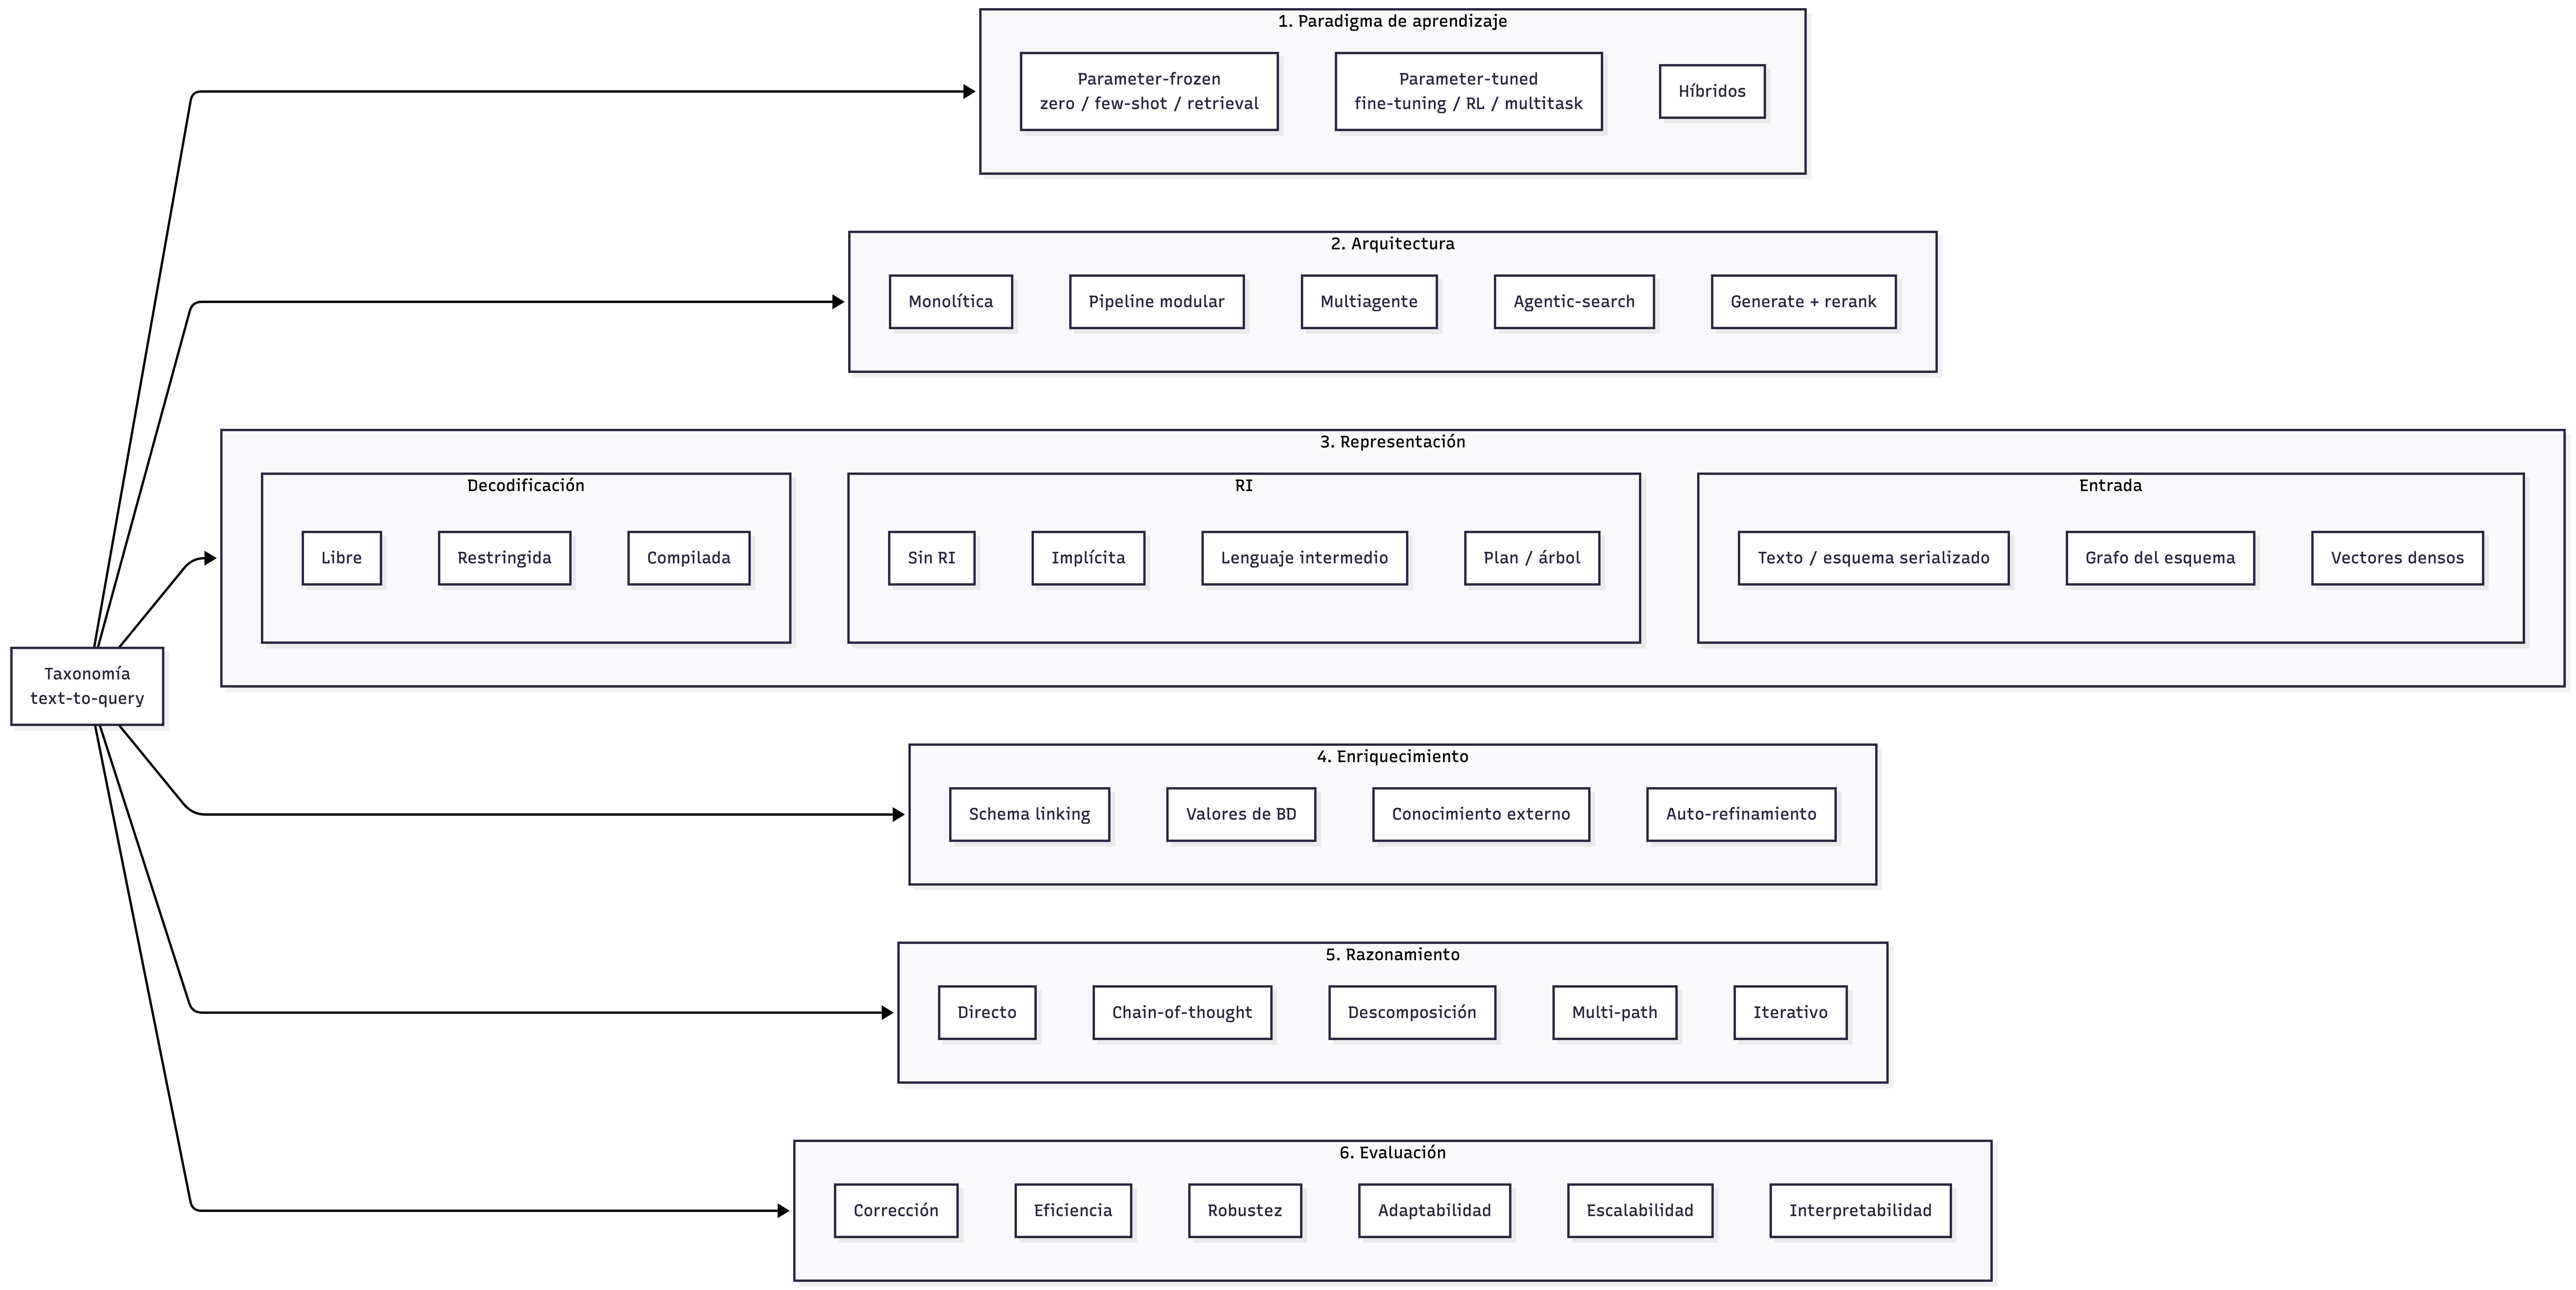
\includegraphics[width=\linewidth]{figs/Chap3/Taxonomía.png}
    \caption{Taxonomía multidimensional propuesta. Cada uno de los seis ejes
    ortogonales agrupa las decisiones de diseño observadas en la literatura
    de \emph{text-to-query} y sus principales subcategorías.}
    \label{fig:taxonomia}
\end{figure}

La Figura~\ref{fig:taxonomia} sintetiza las seis dimensiones consideradas,
cuya descripción y justificación se resumen a continuación:

\begin{enumerate}
    \item \textbf{Paradigma de aprendizaje:} Abarca cómo se adapta el modelo base a la tarea, ya sea con parámetros congelados (\emph{zero-shot}, \emph{few-shot} estático o con recuperación dinámica), parámetros ajustados (\emph{fine-tuning}, preentrenamiento continuo, aprendizaje multi-tarea o por refuerzo) o estrategias híbridas. Esta dimensión ayuda a determinar el costo de adaptación, la dependencia de datos anotados y la complejidad de transferencia a nuevos dominios.

    \item \textbf{Arquitectura del sistema:} La distribución de la ejecución entre el modelo y los diferentes módulos auxiliares, distinguiendo configuraciones monolíticas, \emph{pipelines} modulares, multiagente, \emph{agentic-search} y generación con reordenamiento.

    \item \textbf{Representación:} Las estructuras que median entre la pregunta y la consulta final, considerando codificación de la entrada, representación intermedia y estrategia de decodificación.

    \item \textbf{Mecanismos de enriquecimiento contextual:} La información adicional que ancla la salida al esquema y al dominio, incluyendo \emph{schema linking}, recuperación de contenido de la base de datos, conocimiento externo o ciclos de auto-refinamiento. Se trata como dimensión propia porque su efecto sobre la corrección actúa de forma transversal a la arquitectura y al paradigma de aprendizaje.

    \item \textbf{Paradigma de razonamiento:} Cómo se estructura la inferencia que lleva a la consulta, en variantes directa, en cadena de pensamiento, descompositiva, de múltiples caminos o de retroalimentación iterativa.

    \item \textbf{Evaluación:} Las propiedades del sistema que prioriza explícitamente cada trabajo, entre corrección, eficiencia, robustez, adaptabilidad, escalabilidad e interpretabilidad. Se incorpora como eje independiente para hacer visible el sesgo dominante hacia la corrección y permitir comparaciones sobre propiedades críticas en consultas empresariales.
\end{enumerate}

A partir de esta categorización, las siguientes secciones revisarán la literatura reciente analizando, por dimensión, cómo se han posicionado los trabajos más representativos, enfocándose en propuestas publicadas mayoritariamente entre 2017 y 2026, abarcando de esta forma, desde los primeros sistemas neuronales basados en codificadores especializados hasta las arquitecturas multiagente más recientes.

\section{Paradigma de aprendizaje}
\label{sec:sota-d1-aprendizaje}

Esta sección analiza la forma en que los sistemas \emph{text-to-query} adaptan su modelo base a la tarea, ya que si bien la mayoría de los trabajos revisados utiliza \acp{LLM} o modelos preentrenados de tipo \emph{encoder-decoder}, no todos los sistemas los emplean de la misma manera.









En términos generales, pueden distinguirse tres estrategias principales: La primera consiste en mantener los parámetros del modelo congelados y adaptar su comportamiento únicamente mediante el \emph{prompt}. La segunda ajusta los parámetros del modelo mediante \emph{fine-tuning} u otros procesos de entrenamiento adicional. La tercera combina ambas aproximaciones, por ejemplo, usando modelos congelados para ciertas etapas del \emph{pipeline} y componentes ajustados para tareas específicas como selección, reordenamiento o verificación.

Esta distinción es relevante porque cada estrategia implica compromisos distintos en términos de costo de adaptación, necesidad de datos anotados, flexibilidad frente a nuevos dominios y control sobre el comportamiento del sistema.

\subsection{Aprendizaje con parámetros congelados}
\label{subsec:sota-d1-frozen}

En esta categoría, la adaptación a la tarea se realiza únicamente mediante el diseño del \emph{prompt}, sin modificar los parámetros internos del modelo. Por tanto, la diferencia principal entre los enfoques no está en el entrenamiento del modelo, sino en la forma en que se construye el contexto que se entrega para generar la consulta.

\paragraph{(a) \emph{Zero-shot}.} 
Los enfoques \emph{zero-shot} prescinden de ejemplos demostrativos y se apoyan solo en la pregunta del usuario, la descripción del esquema y las instrucciones incluidas en el \emph{prompt}. C3-SQL~\cite{C3-SQL2023} es representativo de esta línea, ya que muestra que un \emph{prompt} cuidadosamente diseñado puede alcanzar resultados competitivos sobre Spider sin incorporar ejemplos previos. De manera similar, Alpha-SQL~\cite{Alpha-SQL2025}, aunque corresponde a una arquitectura agéntica, puede considerarse \emph{zero-shot} porque no depende de demostraciones específicas del dominio; en su lugar, explora el espacio de consultas mediante búsqueda guiada sobre \emph{prompts} dinámicos.

La principal ventaja de esta subcategoría es su bajo costo de adaptación, pues no requiere datos anotados ni selección de ejemplos. Sin embargo, su desempeño depende fuertemente de la capacidad del modelo base y tiende a degradarse cuando el esquema es grande, poco convencional o presenta relaciones difíciles de inferir solo a partir de su descripción.

\paragraph{(b) \emph{Few-shot in-context learning}.} 
La mayoría de los sistemas recientes basados en \acp{LLM} se ubica en esta subcategoría. En estos enfoques, el modelo recibe un conjunto de ejemplos de pares pregunta-consulta que ilustran el comportamiento esperado. Estos ejemplos pueden ayudar al modelo a reconocer patrones de formulación, estructuras frecuentes de consulta y formas adecuadas de vincular la pregunta con el esquema.

DIN-SQL~\cite{DIN-SQL2023} es uno de los trabajos influyentes en esta línea. Su propuesta descompone la tarea en subpasos y diseña \emph{prompts} específicos para cada uno, apoyados en ejemplos seleccionados manualmente. Enfoques posteriores o relacionados, como DAIL-SQL~\cite{DAIL-SQL2023}, ACT-SQL~\cite{ACT-SQL2023}, PET-SQL~\cite{PET-SQL2024}, DEA-SQL~\cite{DEA-SQL2024}, RSL-SQL~\cite{RSL-SQL2024}, CHESS~\cite{CHESS2024}, MAC-SQL~\cite{MAC-SQL2023}, TA-SQL~\cite{TA-SQL2024}, CoE-SQL~\cite{CoE-SQL2024}, PURPLE~\cite{PURPLE2024}, ODIS~\cite{ODIS2023}, Gen-SQL~\cite{Gen-SQL2025}, SGU-SQL~\cite{SGU-SQL2025}, CRED-SQL~\cite{CRED-SQL2025} y CRUSH4SQL~\cite{CRUSH4SQL2023}, entre otros, mantienen esta lógica general, aunque la combinan con distintas formas de descomposición, recuperación, verificación o refinamiento.

La amplitud de trabajos en esta subcategoría muestra la madurez del paradigma de aprendizaje en contexto. No obstante, también evidencia una limitación: muchas mejoras dependen de ajustes en la ingeniería de \emph{prompts}, la selección de ejemplos o la organización del contexto, más que de cambios profundos en la arquitectura del sistema.

\paragraph{(c) Aprendizaje en contexto dinámico con recuperación.} 
Una variante más flexible del \emph{few-shot} consiste en seleccionar dinámicamente los ejemplos que se incluyen en el \emph{prompt}. En lugar de usar un conjunto fijo de demostraciones, el sistema recupera ejemplos similares a la pregunta de entrada o al esquema objetivo. Esta estrategia busca que el contexto proporcionado al modelo sea más relevante para cada caso particular.

OpenSearch-SQL~\cite{OpenSearch-SQL2025} ilustra esta aproximación mediante un módulo dedicado a la recuperación de ejemplos. CRED-SQL~\cite{CRED-SQL2025} también contempla esta estrategia como una extensión posible dentro de su arquitectura. La ventaja principal frente al \emph{few-shot} estático es su mayor adaptabilidad a dominios heterogéneos. Sin embargo, esta adaptabilidad depende de la calidad, cobertura y organización del corpus de ejemplos disponible. Si los ejemplos recuperados son poco representativos o introducen patrones incorrectos, el desempeño del modelo puede verse afectado.

\subsection{Aprendizaje con parámetros ajustados}
\label{subsec:sota-d1-tuned}

En esta categoría se modifican los parámetros del modelo mediante
entrenamiento adicional sobre datos específicos de la tarea. Es la familia
históricamente más extendida en \emph{text-to-SQL} previa al auge de los
\acp{LLM} de propósito general.

\paragraph{(a) Fine-tuning supervisado.} Trabajos como
Seq2SQL~\cite{Seq2SQL2017}, BRIDGE~\cite{BRIDGE2020},
RAT-SQL~\cite{RAT-SQL2021}, SmBoP~\cite{SmBoP2021},
RaSaP~\cite{RaSaP2021}, SHiP~\cite{SHiP2022},
RASAT~\cite{RASAT2022}, PICARD~\cite{PICARD2022},
S²SQL~\cite{S2SQL2022}, Graphix-T5~\cite{Graphix-T52022},
RESDSQL~\cite{RESDSQL2023}, T5-3B+NatSQL~\cite{T5-3B+NatSQL+TokenPreprocessing2023},
SQLFormer~\cite{SQLFormer2023}, CatSQL~\cite{CatSQL2023} y
DTS-SQL~\cite{DTS-SQL2024} ajustan modelos completos sobre conjuntos como
Spider o WikiSQL. Las arquitecturas base varían desde redes específicas para
\emph{text-to-SQL} (Seq2SQL, BRIDGE, RAT-SQL, SmBoP) hasta variantes de T5
adaptadas (PICARD, RESDSQL, Graphix-T5). Los sistemas de esta sub-categoría
dominaron los rankings de los benchmarks controlados durante el período
pre-LLM (2017--2022); su costo de entrenamiento y su dependencia del dominio
de entrenamiento limitan, sin embargo, su transferencia directa a entornos
empresariales.

\paragraph{(b) Preentrenamiento continuo.} CodeS~\cite{CodeS2024} representa
una variante intermedia: parte de un modelo de código preentrenado de
propósito general y aplica preentrenamiento continuo sobre un corpus
masivo orientado a SQL antes del \emph{fine-tuning} supervisado final. La
estrategia mejora la transferencia a dominios desconocidos, pero requiere
infraestructura considerable y un corpus de entrenamiento curado.

\paragraph{(c) Aprendizaje multi-tarea.} Algunos trabajos entrenan el modelo
sobre varias tareas relacionadas para mejorar la generalización.
TKK~\cite{TKK2022} aborda \emph{text-to-SQL} junto con tareas auxiliares
de comprensión de esquema. ROUTE~\cite{ROUTE2025} adopta el aprendizaje
multi-tarea como principio organizador del \emph{fine-tuning},
integrando tareas de generación, corrección y razonamiento sobre esquemas.
PARSQL~\cite{PARSQL2025} sigue una línea similar al combinar generación con
selección entre candidatos. La motivación común es que las tareas auxiliares
fuerzan al modelo a desarrollar representaciones internas más robustas del
esquema y de la sintaxis SQL.

\paragraph{(d) Aprendizaje por refuerzo.} STRuCT-LLM~\cite{STRuCT-LLM2025}
incorpora aprendizaje por refuerzo para alinear la generación con
señales de ejecución y con tareas de razonamiento sobre tablas y grafos
simultáneamente. Seq2SQL~\cite{Seq2SQL2017}, en una época mucho más
temprana, ya empleaba aprendizaje por refuerzo basado en la recompensa de
ejecución. La adopción del paradigma sigue siendo minoritaria pero ha
resurgido con fuerza en propuestas recientes orientadas a unificar
razonamiento estructurado con generación.

\subsection{Estrategias híbridas}
\label{subsec:sota-d1-hibridas}

Una fracción creciente de los sistemas más recientes combina componentes
con parámetros congelados y componentes ajustados.
XiYan-SQL~\cite{XiYan-SQL2024} adopta una arquitectura multiagente en la que
un generador puede ser un \ac{LLM} ajustado de la familia
XiYanSQL-QwenCoder mientras que módulos auxiliares operan
\emph{in-context}. CHASE-SQL~\cite{CHASE-SQL2025} combina generadores
\emph{in-context} con un seleccionador entrenado mediante \emph{fine-tuning}.
ZeroNL2SQL~\cite{ZeroNL2SQL2024} distribuye la carga entre un modelo
preentrenado pequeño y un \ac{LLM} congelado. MetaSQL~\cite{MetaSQL2024}
aplica un esquema análogo en la fase de selección sobre múltiples
candidatos. La motivación es pragmática: aprovechar la capacidad de
generalización de los \acp{LLM} sin renunciar al control fino que provee
el ajuste sobre los componentes críticos.

\subsection{Observaciones críticas}
\label{subsec:sota-d1-obs}

La revisión de esta dimensión muestra un desplazamiento progresivo del
\emph{fine-tuning} de extremo a extremo hacia configuraciones híbridas
y \emph{in-context}. Esta tendencia es coherente con el aumento del costo
computacional asociado al entrenamiento de \acp{LLM} de gran tamaño. Sin
embargo, los sistemas puramente \emph{in-context} acumulan dos
limitaciones recurrentes: dependencia fuerte del modelo subyacente, lo
que dificulta auditar el sistema desde el punto de vista de gobernanza, y
ausencia de mecanismos formales para garantizar que la salida respete
el esquema. La investigación de la presente tesis se posiciona como
agnóstica al paradigma de aprendizaje subyacente: el énfasis se traslada
a la representación intermedia y al bucle de verificación, de modo que
la corrección estructural no descanse exclusivamente en la calidad
estadística del generador.

\section{Arquitectura del Sistema}
\label{sec:sota-d2-arquitectura}

Esta sección describe cómo se organiza el cómputo en los sistemas
\emph{text-to-query}. La distinción es independiente del paradigma de
aprendizaje: un mismo paradigma puede dar lugar a arquitecturas
monolíticas, modulares, multiagente, agénticas o de generación con
reordenamiento.

\subsection{Arquitecturas monolíticas}
\label{subsec:sota-d2-monoliticas}

En las arquitecturas monolíticas, una sola invocación del modelo produce
la consulta completa. Es la configuración natural de los sistemas
\emph{end-to-end} entrenados para mapear pregunta a consulta directamente.
Pertenecen a esta categoría Seq2SQL~\cite{Seq2SQL2017},
BRIDGE~\cite{BRIDGE2020}, RAT-SQL~\cite{RAT-SQL2021},
SmBoP~\cite{SmBoP2021}, RaSaP~\cite{RaSaP2021}, RASAT~\cite{RASAT2022},
PICARD~\cite{PICARD2022}, S²SQL~\cite{S2SQL2022},
Graphix-T5~\cite{Graphix-T52022}, T5-3B+NatSQL~\cite{T5-3B+NatSQL+TokenPreprocessing2023},
SQLFormer~\cite{SQLFormer2023}, CatSQL~\cite{CatSQL2023},
SHiP~\cite{SHiP2022}, CodeS~\cite{CodeS2024},
DAIL-SQL~\cite{DAIL-SQL2023}, ACT-SQL~\cite{ACT-SQL2023},
ODIS~\cite{ODIS2023}, SGU-SQL~\cite{SGU-SQL2025} y
STRuCT-LLM~\cite{STRuCT-LLM2025}. Aunque algunos de estos sistemas
internamente realizan operaciones de codificación o decodificación
sofisticadas, conceptualmente la generación de la consulta es una sola
inferencia. La ventaja principal de esta organización es la simplicidad
operativa; la desventaja es que cualquier error se propaga sin posibilidad
de inspección intermedia ni de intervención modular.

\subsection{Pipelines modulares}
\label{subsec:sota-d2-pipelines}

En esta categoría, la generación se distribuye entre etapas secuenciales
con responsabilidades distintas: típicamente \emph{schema linking},
generación, validación y refinamiento. DIN-SQL~\cite{DIN-SQL2023} popularizó
una variante influyente del enfoque, descomponiendo el proceso en cuatro
sub-tareas. La línea ha sido seguida por numerosos trabajos:
RESDSQL~\cite{RESDSQL2023}, DTS-SQL~\cite{DTS-SQL2024},
PURPLE~\cite{PURPLE2024}, RSL-SQL~\cite{RSL-SQL2024},
DEA-SQL~\cite{DEA-SQL2024}, CoE-SQL~\cite{CoE-SQL2024},
PET-SQL~\cite{PET-SQL2024}, SuperSQL~\cite{SuperSQL2024},
TA-SQL~\cite{TA-SQL2024}, FinSQL~\cite{FinSQL2024},
TKK~\cite{TKK2022}, ZeroNL2SQL~\cite{ZeroNL2SQL2024},
SteinerSQL~\cite{SteinerSQL2025}, Gen-SQL~\cite{Gen-SQL2025},
BLENDSQL~\cite{BLENDSQL2025}, CRED-SQL~\cite{CRED-SQL2025},
CRUSH4SQL~\cite{CRUSH4SQL2023}, SelECT-SQL~\cite{SC-Prompt2023},
CHESS~\cite{CHESS2024}, C3-SQL~\cite{C3-SQL2023} y
Wren AI~\cite{WrenAI2025}. Los \emph{pipelines} modulares facilitan la
inspección, el reemplazo de componentes y la integración con sistemas de
verificación, lo que los hace especialmente atractivos para entornos
empresariales. Su limitación principal es la rigidez del orden de
ejecución y la posible amplificación de errores entre etapas.

\subsection{Arquitecturas multiagente}
\label{subsec:sota-d2-multiagente}

Una variante reciente del enfoque modular dota a cada componente de
autonomía e iniciativa, configurándolo como un agente que se comunica con
otros mediante mensajes. MAC-SQL~\cite{MAC-SQL2023} es uno de los
trabajos influyentes en consolidar esta organización para \emph{text-to-SQL},
con agentes especializados en \emph{schema linking}, descomposición y
refinamiento. CHESS~\cite{CHESS2024} extiende esta línea con cuatro
agentes ---recuperación de información, selección de esquema, generación
y verificación--- e incorpora un agente \emph{Unit Tester} que actúa como
verificador semántico. OpenSearch-SQL~\cite{OpenSearch-SQL2025} y
TS-SQL~\cite{TS-SQL2025} adoptan también una organización multiagente.
XiYan-SQL~\cite{XiYan-SQL2024} combina varios agentes generadores con un
agente seleccionador. La diferencia operativa entre un \emph{pipeline}
modular y un sistema multiagente es a menudo gradual; en la práctica, lo
distintivo del enfoque multiagente es la capacidad de varios componentes
de invocar al modelo de forma asíncrona o cíclica.

\subsection{Arquitecturas agentic-search}
\label{subsec:sota-d2-agentic}

Algunos trabajos abandonan la idea de un orden fijo y adoptan en su lugar
una exploración guiada del espacio de soluciones.
Alpha-SQL~\cite{Alpha-SQL2025} ilustra esta categoría: utiliza un modelo
para proponer acciones (refinar el esquema, generar un fragmento, verificar
una sub-consulta) y un mecanismo de búsqueda para decidir qué acción
ejecutar a continuación. CHASE-SQL~\cite{CHASE-SQL2025} también incorpora
elementos de exploración, aunque combinados con generación múltiple. La
ventaja del enfoque es su flexibilidad ante consultas complejas; su
desventaja, el costo computacional asociado a la búsqueda y la dificultad
de garantizar terminación.

\subsection{Arquitecturas de generación con reordenamiento}
\label{subsec:sota-d2-rerank}

En esta categoría, el sistema produce varios candidatos de consulta y un
módulo posterior selecciona el mejor. CHASE-SQL~\cite{CHASE-SQL2025},
XiYan-SQL~\cite{XiYan-SQL2024} y MetaSQL~\cite{MetaSQL2024} adoptan
explícitamente esta estrategia. PARSQL~\cite{PARSQL2025} también opera
sobre un conjunto de candidatos y G\textsuperscript{3}R~\cite{G3R2023}
incorpora una etapa de reordenamiento basada en alineación. Trabajos
clásicos como N-best List Rerankers~\cite{N-bestListRerankers2022} sentaron
las bases del enfoque. La motivación es robusta: si el generador produce un
candidato correcto entre varios, un reordenador entrenado puede
recuperarlo aún cuando no sea el más probable a priori. La debilidad es la
dependencia de la diversidad real del conjunto generado.

\subsection{Observaciones críticas}
\label{subsec:sota-d2-obs}

La distribución de los trabajos analizados por arquitectura muestra una
migración progresiva desde sistemas monolíticos ---propios de la era
\emph{pre-LLM}--- hacia \emph{pipelines} modulares, multiagente y
agénticos. Esta evolución responde tanto a la creciente complejidad de las
consultas objetivo como a la necesidad de inspeccionar y verificar la
salida en entornos críticos. Sin embargo, una limitación común a las
arquitecturas modulares y multiagente es que la verificación semántica,
cuando existe, suele ejecutarse al final del proceso sobre la consulta ya
generada, y rara vez se realiza sobre una representación intermedia que
admita análisis estático. Esta brecha es uno de los puntos que la
propuesta de la presente tesis aborda explícitamente.

\section{Estrategias de Representación}
\label{sec:sota-d3-representacion}

La forma en que un sistema representa la pregunta, el esquema y la
consulta en formación condiciona qué tipos de errores puede detectar y
qué tipos de control puede ejercer sobre la salida. Esta sección agrupa
los trabajos según los tres ejes complementarios de la dimensión:
codificación de la entrada, representación intermedia entre comprensión y
generación, y estrategia de decodificación de la consulta final.

\subsection{Codificación de la entrada}
\label{subsec:sota-d3a-encoding}

\paragraph{(a) Esquema serializado en lenguaje natural.} La práctica
dominante en sistemas basados en \acp{LLM} consiste en serializar el
esquema como un fragmento de texto que se concatena con la pregunta.
DIN-SQL~\cite{DIN-SQL2023}, DAIL-SQL~\cite{DAIL-SQL2023},
ACT-SQL~\cite{ACT-SQL2023}, MAC-SQL~\cite{MAC-SQL2023},
CHESS~\cite{CHESS2024} y la mayoría de los sistemas \emph{in-context}
recientes emplean esta codificación. Su ventaja es la simplicidad y la
compatibilidad universal con \acp{LLM}; su desventaja es que se pierden
las relaciones estructurales del esquema, salvo que se reintroduzcan
explícitamente en el texto.

\paragraph{(b) Grafos del esquema.} Una línea de trabajos modela
explícitamente el esquema como un grafo, donde los nodos representan
tablas y columnas y las aristas representan claves foráneas y otras
relaciones. RAT-SQL~\cite{RAT-SQL2021}, S²SQL~\cite{S2SQL2022} y
Graphix-T5~\cite{Graphix-T52022} incorporan capas de atención sensibles
a la estructura del grafo. La motivación es facilitar el razonamiento
sobre uniones complejas y rutas de \emph{join} no triviales. El costo
es una mayor complejidad arquitectónica y la necesidad de construir el
grafo del esquema como paso de preprocesamiento.

\paragraph{(c) Esquema enriquecido (M-Schema y similares).}
XiYan-SQL~\cite{XiYan-SQL2024} introduce M-Schema, un formato que
combina el esquema con metadatos y ejemplos de valores en una
representación textual estructurada que el \ac{LLM} consume directamente.
Esta codificación intermedia entre texto plano y grafo busca preservar
la simplicidad del primero sin perder la información estructural del
segundo. Otros trabajos, como CHESS~\cite{CHESS2024} y
PET-SQL~\cite{PET-SQL2024}, adoptan formatos análogos en su etapa de
preparación del \emph{prompt}.

\paragraph{(d) Recuperación previa al modelo.} En esquemas masivos, no
es viable serializar el esquema completo en el \emph{prompt}.
CRUSH4SQL~\cite{CRUSH4SQL2023} aborda esta restricción mediante
recuperación: un módulo previo selecciona los elementos del esquema
relevantes para la pregunta antes de invocar al modelo.
TS-SQL~\cite{TS-SQL2025} y SuperSQL~\cite{SuperSQL2024} contemplan
estrategias análogas. El compromiso es entre cobertura ---no omitir
elementos críticos--- y compacidad ---no saturar el contexto.

\subsection{Representación intermedia}
\label{subsec:sota-d3b-ir}

Esta sub-dimensión es central para la presente tesis. Se distinguen seis
sub-categorías según el tipo de RI que cada sistema utiliza, si es que
utiliza alguna.

\paragraph{(a) Sin RI explícita.} La consulta se genera directamente como
secuencia de tokens del lenguaje destino. Pertenecen a esta categoría
Seq2SQL~\cite{Seq2SQL2017}, BRIDGE~\cite{BRIDGE2020},
DAIL-SQL~\cite{DAIL-SQL2023}, ACT-SQL~\cite{ACT-SQL2023},
ODIS~\cite{ODIS2023}, SuperSQL~\cite{SuperSQL2024} y la mayoría de los
sistemas \emph{in-context} basados en \emph{prompting}. La ausencia de
RI explícita simplifica la arquitectura, pero traslada toda la carga de
corrección estructural al generador.

\paragraph{(b) Esquema como RI implícita.} Algunos trabajos no introducen
una RI dedicada, pero usan el esquema enriquecido como sustrato sobre el
cual se realiza el razonamiento previo a la generación. Es el caso de
RAT-SQL~\cite{RAT-SQL2021} y, en parte, de XiYan-SQL~\cite{XiYan-SQL2024}
con su M-Schema. La consulta sigue siendo SQL nativo, pero la
representación del esquema actúa como puente estructurado.

\paragraph{(c) Lenguaje intermedio dedicado.} La línea más explícita
hacia una RI propiamente dicha la inicia IRNet con SemQL~\cite{guo2019irnet}, un
lenguaje intermedio que separa interpretación semántica de sintaxis SQL
concreta. NatSQL~\cite{gan2021natsql} sigue una motivación análoga:
define un lenguaje SQL simplificado sobre el que se entrena el modelo, y
un compilador trivial lo convierte a SQL ejecutable. El trabajo
T5-3B+NatSQL~\cite{T5-3B+NatSQL+TokenPreprocessing2023} se apoya
directamente sobre esta \ac{RI} para mejorar la generalización. CatSQL~\cite{CatSQL2023} y ZeroNL2SQL~\cite{ZeroNL2SQL2024}
contemplan formas similares de representación intermedia. La ventaja
estructural es que la RI restringe el espacio de errores posibles del
modelo; la limitación es que la RI suele estar acoplada a un dialecto
específico de SQL.

\paragraph{(d) Plan estructurado.} Algunos sistemas representan la
consulta como un plan de ejecución o como una secuencia de operaciones
declarativas. SQLFormer~\cite{SQLFormer2023} sigue parcialmente esta
línea al organizar la generación alrededor de operaciones primitivas.
SteinerSQL~\cite{SteinerSQL2025} representa la consulta como un árbol
sobre el grafo del esquema, lo que se aproxima a una representación
plan-céntrica. La ventaja es la trazabilidad del razonamiento; la
limitación es el costo de adoptar y mantener un formalismo propio.

\paragraph{(e) Árbol abstracto.} SmBoP~\cite{SmBoP2021} construye la
consulta de forma composicional como un árbol abstracto sobre operadores
relacionales, generando \emph{bottom-up}. PICARD~\cite{PICARD2022} no
expone explícitamente un árbol como artefacto, pero su decodificación
restringida opera implícitamente sobre la gramática del lenguaje, lo
que lo posiciona en una categoría afín. RaSaP~\cite{RaSaP2021} y
SQLFormer~\cite{SQLFormer2023} también incorporan estructura arbórea en
distintos grados.

\paragraph{(f) Descomposición declarativa.}
DIN-SQL~\cite{DIN-SQL2023} introduce una forma específica de RI
implícita: la pregunta se descompone en sub-preguntas y cada
sub-pregunta produce una sub-consulta, que luego se ensambla. La
descomposición no es una RI estructural, pero juega un papel análogo al
distribuir el razonamiento. CHESS~\cite{CHESS2024} y
MAC-SQL~\cite{MAC-SQL2023} adoptan estrategias similares.

\subsection{Estrategias de decodificación}
\label{subsec:sota-d3c-decoding}

\paragraph{(a) Decodificación libre.} El modelo genera la consulta como
texto sin restricciones formales. Es la estrategia dominante en sistemas
\emph{in-context}: DIN-SQL~\cite{DIN-SQL2023}, DAIL-SQL~\cite{DAIL-SQL2023},
ACT-SQL~\cite{ACT-SQL2023}, CHESS~\cite{CHESS2024},
MAC-SQL~\cite{MAC-SQL2023}, OpenSearch-SQL~\cite{OpenSearch-SQL2025},
XiYan-SQL~\cite{XiYan-SQL2024}, entre otros. Su ventaja es la
flexibilidad; su desventaja, la posibilidad de generar consultas
sintácticamente inválidas.

\paragraph{(b) Decodificación restringida por gramática.}
PICARD~\cite{PICARD2022} establece el patrón de referencia de esta
categoría: integra una gramática de SQL en el decodificador para
descartar en tiempo real candidatos que violen el lenguaje. La técnica
elimina por completo los errores sintácticos al costo de una
decodificación más cara. PICARD inspira aplicaciones posteriores en
otros componentes de \emph{pipelines} modulares.

\paragraph{(c) Decodificación composicional.} SmBoP~\cite{SmBoP2021}
genera la consulta de manera \emph{bottom-up} sobre operadores
relacionales, imponiendo estructura desde el inicio de la derivación.
La estrategia es más compleja de implementar pero garantiza por
construcción ciertos invariantes estructurales.

\paragraph{(d) Compilación desde la representación intermedia.} Cuando
el sistema utiliza una RI explícita, la decodificación final puede
reducirse a la compilación determinista de la RI al lenguaje destino.
IRNet~\cite{guo2019irnet} y NatSQL~\cite{gan2021natsql}
operan así: el modelo genera la RI y un componente determinista produce
la consulta. Esta estrategia separa por completo el riesgo estadístico
del riesgo formal.

\subsection{Observaciones críticas}
\label{subsec:sota-d3-obs}

La revisión muestra que la mayoría de los sistemas recientes basados en
\acp{LLM} ha priorizado simplificar la representación ---esquema
serializado, decodificación libre, sin RI explícita--- delegando la
corrección al generador. Esta decisión ha sido razonable mientras los
benchmarks dominantes contenían esquemas de complejidad moderada y
consultas SQL relativamente regulares. Sin embargo, en escenarios
empresariales y, especialmente, en consultas híbridas sobre el estándar
\ac{SQL}/\ac{PGQ}, la ausencia de RI explícita amplifica la propagación
de alucinaciones estructurales: no existe una capa intermedia donde
verificar la consistencia de tipos, la validez de las uniones o la
coherencia entre los componentes relacionales y de patrón de grafo.
La investigación de esta tesis se posiciona deliberadamente en la
sub-categoría de RI explícita con compilación determinista, ampliada
para cubrir tanto SQL como PGQ y enriquecida con verificación estática
sobre la propia RI.

\section{Mecanismos de Enriquecimiento Contextual}
\label{sec:sota-d4-enriquecimiento}

Esta sección agrupa las técnicas que aportan información adicional al
modelo más allá de la pregunta y el esquema básico. Los cuatro
mecanismos no son excluyentes: muchos sistemas combinan varios.

\subsection{Schema linking}
\label{subsec:sota-d4-schemalinking}

El \emph{schema linking} consiste en establecer correspondencias
explícitas entre menciones del texto y elementos del esquema (tablas,
columnas, valores). Esta operación es central en \emph{text-to-SQL} y ha
recibido tratamiento dedicado tanto como módulo independiente como
integrado dentro de la arquitectura. RAT-SQL~\cite{RAT-SQL2021} la
incorpora mediante atención sensible a relaciones del esquema.
RESDSQL~\cite{RESDSQL2023}, DTS-SQL~\cite{DTS-SQL2024},
DIN-SQL~\cite{DIN-SQL2023}, DEA-SQL~\cite{DEA-SQL2024},
RSL-SQL~\cite{RSL-SQL2024}, CHESS~\cite{CHESS2024},
MAC-SQL~\cite{MAC-SQL2023}, TA-SQL~\cite{TA-SQL2024},
PURPLE~\cite{PURPLE2024}, TS-SQL~\cite{TS-SQL2025} y
CRUSH4SQL~\cite{CRUSH4SQL2023}, entre otros, dedican un módulo o etapa
específica al \emph{schema linking}. La calidad de esta etapa se
correlaciona fuertemente con la corrección final del sistema, lo que
explica la atención sostenida que ha recibido.

\subsection{Recuperación de contenido de la base de datos}
\label{subsec:sota-d4-content}

Algunos sistemas incorporan valores reales de las columnas para resolver
ambigüedades léxicas que el esquema solo no permite resolver
---por ejemplo, distinguir entre dos columnas con nombres similares pero
contenido distinto. BRIDGE~\cite{BRIDGE2020} fue uno de los primeros en
hacerlo de forma sistemática. Trabajos posteriores como
CHESS~\cite{CHESS2024}, FinSQL~\cite{FinSQL2024},
PET-SQL~\cite{PET-SQL2024}, CHASE-SQL~\cite{CHASE-SQL2025},
CRED-SQL~\cite{CRED-SQL2025} y SuperSQL~\cite{SuperSQL2024} adoptan
estrategias análogas, recuperando muestras de valores relevantes para la
pregunta. La eficacia depende de la calidad del proceso de recuperación
y plantea desafíos cuando los datos contienen información sensible.

\subsection{Conocimiento externo y de dominio}
\label{subsec:sota-d4-external}

En entornos empresariales, una fracción significativa de las consultas
no puede resolverse correctamente sin conocimiento externo: glosarios de
métricas, definiciones de dominio, restricciones de negocio. La línea
de trabajos que aborda esta necesidad es comparativamente menor pero
relevante. atscale2024sml~\cite{atscale2024sml} ilustra el uso de un
\emph{semantic layer} corporativo. SAFENLIDB~\cite{SAFENLIDB} aborda el
componente de privacidad y seguridad de la integración con conocimiento
externo. ROUTE~\cite{ROUTE2025} incorpora señales de robustez que
implícitamente requieren conocimiento adicional sobre el dominio.
La principal limitación de esta categoría es la falta de
estandarización: cada trabajo define su propio formato para representar
el conocimiento externo, lo que dificulta la comparación.

\subsection{Auto-refinamiento}
\label{subsec:sota-d4-refinement}

Una proporción creciente de sistemas incorpora ciclos en los que la
consulta generada se ejecuta o se inspecciona, y los resultados o los
errores se reintroducen al modelo para corrección.
DIN-SQL~\cite{DIN-SQL2023} incluye una etapa de auto-corrección.
MAC-SQL~\cite{MAC-SQL2023}, CHESS~\cite{CHESS2024},
XiYan-SQL~\cite{XiYan-SQL2024}, OpenSearch-SQL~\cite{OpenSearch-SQL2025},
DEA-SQL~\cite{DEA-SQL2024}, RSL-SQL~\cite{RSL-SQL2024},
PURPLE~\cite{PURPLE2024} y CHASE-SQL~\cite{CHASE-SQL2025} adoptan
variantes de este mecanismo. Los trabajos sobre detección de errores
---ErrorLLM~\cite{errorllm2026}, SQLHD~\cite{SQLHD2025},
AmbiSQL~\cite{AmbiSQL}--- proveen señales que, en principio, podrían
alimentar el bucle de auto-refinamiento. La eficacia del mecanismo
depende crucialmente de la naturaleza de la retroalimentación: cuando
es texto libre, tiende a inducir oscilaciones; cuando es estructurada,
puede converger más rápidamente.

\subsection{Observaciones críticas}
\label{subsec:sota-d4-obs}

El \emph{schema linking} es el mecanismo más estudiado, mientras que la
integración de conocimiento externo de dominio es claramente el menos
desarrollado pese a su relevancia empresarial directa. El
auto-refinamiento ha proliferado, pero la mayoría de las
implementaciones operan sobre la consulta final como texto, lo que
limita la precisión de la corrección posible y dificulta su análisis
sistemático. Una arquitectura que opere sobre una RI tipada permite
sustituir el bucle de auto-corrección sobre texto por
retroalimentación estructurada que actúe sobre el nodo o la condición
exacta donde se detectó el error.

\section{Paradigma de Razonamiento}
\label{sec:sota-d5-razonamiento}

Esta sección agrupa los sistemas según cómo estructuran el proceso de
inferencia que conduce de la pregunta a la consulta. El paradigma de
razonamiento es independiente de la arquitectura del sistema: una
arquitectura monolítica puede emplear razonamiento directo o en cadena,
y un \emph{pipeline} modular puede operar de forma descompositiva o
iterativa.

\subsection{Razonamiento directo}
\label{subsec:sota-d5-directo}

El modelo produce la consulta sin pasos intermedios explícitos. Es la
estrategia natural en sistemas \emph{end-to-end}:
Seq2SQL~\cite{Seq2SQL2017}, BRIDGE~\cite{BRIDGE2020},
RAT-SQL~\cite{RAT-SQL2021}, RASAT~\cite{RASAT2022},
PICARD~\cite{PICARD2022}, Graphix-T5~\cite{Graphix-T52022},
RESDSQL~\cite{RESDSQL2023}, T5-3B+NatSQL~\cite{T5-3B+NatSQL+TokenPreprocessing2023}
y CodeS~\cite{CodeS2024}. Estos sistemas confían el razonamiento al
proceso interno del modelo y a las representaciones intermedias
implícitas que aprende durante el entrenamiento.

\subsection{Cadena de pensamiento}
\label{subsec:sota-d5-cot}

Aquí el modelo expone, antes de la consulta, una traza textual del
razonamiento que conduce a ella. ACT-SQL~\cite{ACT-SQL2023} es una
referencia explícita en esta línea, con \emph{prompts} que inducen
\emph{chain-of-thought} adaptado a \emph{text-to-SQL}.
ODIS~\cite{ODIS2023}, DAIL-SQL~\cite{DAIL-SQL2023},
PET-SQL~\cite{PET-SQL2024}, SuperSQL~\cite{SuperSQL2024},
CoE-SQL~\cite{CoE-SQL2024} y CRED-SQL~\cite{CRED-SQL2025} adoptan
variantes del enfoque. La principal limitación es que la traza textual
no es verificable estructuralmente; el modelo puede producir un
razonamiento aparentemente válido y aun así generar una consulta
errónea.

\subsection{Razonamiento descompositivo}
\label{subsec:sota-d5-descompositivo}

La pregunta se divide explícitamente en sub-preguntas, cada una de las
cuales se resuelve por separado y se ensambla luego.
DIN-SQL~\cite{DIN-SQL2023} es la referencia principal en esta línea.
MAC-SQL~\cite{MAC-SQL2023}, CHESS~\cite{CHESS2024},
DEA-SQL~\cite{DEA-SQL2024}, RSL-SQL~\cite{RSL-SQL2024},
TA-SQL~\cite{TA-SQL2024}, SuperSQL~\cite{SuperSQL2024} y
SteinerSQL~\cite{SteinerSQL2025} la adoptan en variantes propias. La
descomposición es coherente con la observación práctica de que las
consultas complejas se resuelven mejor cuando se atacan por partes,
aunque introduce el riesgo de descomposiciones incorrectas que
arrastran errores difíciles de localizar.

\subsection{Razonamiento de múltiples caminos}
\label{subsec:sota-d5-multipath}

El sistema produce varias trayectorias o varios candidatos en paralelo y
elige entre ellos. CHASE-SQL~\cite{CHASE-SQL2025},
XiYan-SQL~\cite{XiYan-SQL2024}, MetaSQL~\cite{MetaSQL2024},
PARSQL~\cite{PARSQL2025}, G\textsuperscript{3}R~\cite{G3R2023} y
N-best List Rerankers~\cite{N-bestListRerankers2022} pertenecen a esta
sub-categoría. La motivación está sustentada por la observación
empírica de que el candidato más probable según el modelo no es
siempre el correcto; la diversidad del conjunto generado actúa como
mecanismo de tolerancia a errores. La dificultad reside en construir un
seleccionador o reordenador que efectivamente identifique el candidato
correcto.

\subsection{Razonamiento de retroalimentación iterativa}
\label{subsec:sota-d5-iterativo}

La consulta se refina en sucesivas iteraciones a partir de
retroalimentación de ejecución, validación o un agente verificador.
CHESS~\cite{CHESS2024} con su Unit Tester, MAC-SQL~\cite{MAC-SQL2023}
con su agente de refinamiento, OpenSearch-SQL~\cite{OpenSearch-SQL2025},
DIN-SQL~\cite{DIN-SQL2023}, RSL-SQL~\cite{RSL-SQL2024},
DEA-SQL~\cite{DEA-SQL2024} y CHASE-SQL~\cite{CHASE-SQL2025} operan en
ciclos iterativos. ErrorLLM~\cite{errorllm2026} y SQLHD~\cite{SQLHD2025}
proveen modelos de detección de errores que pueden alimentar tales
ciclos. AmbiSQL~\cite{AmbiSQL} aborda iterativamente la resolución de
ambigüedades en interacción con el usuario. La efectividad del
paradigma depende de que la retroalimentación sea informativa y
discriminante; en su ausencia, el ciclo puede oscilar sin converger.

\subsection{Observaciones críticas}
\label{subsec:sota-d5-obs}

La descomposición y la retroalimentación iterativa han desplazado al
razonamiento directo en los sistemas más recientes basados en
\acp{LLM}. Sin embargo, la cadena de pensamiento y la descomposición,
en sus implementaciones predominantes, operan sobre texto libre y son
por lo tanto difíciles de auditar y de verificar formalmente. La
investigación de esta tesis explora una estrategia complementaria: la
descomposición y la retroalimentación operan sobre una RI estructurada
y tipada, lo que convierte cada paso del razonamiento en un artefacto
inspectable y verificable mediante reglas explícitas.

\section{Propiedades Evaluativas Objetivo}
\label{sec:sota-d6-propiedades}

Esta sección caracteriza la literatura por las propiedades del sistema
que cada trabajo prioriza explícitamente en su evaluación. Se distinguen
seis propiedades, no excluyentes, que guían el diseño y la
experimentación.

\subsection{Corrección}
\label{subsec:sota-d6-correccion}

La corrección, medida típicamente como exactitud de ejecución
(\emph{execution accuracy}) o coincidencia exacta (\emph{exact match}),
es la propiedad históricamente dominante. Prácticamente todos los
trabajos analizados la reportan: Spider~\cite{spider2_2025},
BIRD~\cite{BIRD2023} y otros benchmarks han consolidado su uso como
métrica de referencia.
La crítica recurrente, presente en
EvaluatingRobustness~\cite{EvaluatingRobustness} y en
NLinterfaces~\cite{NLinterfaces}, es que la exactitud sobre benchmarks
controlados sobreestima el desempeño en entornos reales.

\subsection{Eficiencia}
\label{subsec:sota-d6-eficiencia}

Una fracción menor de trabajos prioriza explícitamente la eficiencia de
la consulta generada, no solo la corrección de su resultado.
CodeScore~\cite{CodeScore} y atscale2024sml~\cite{atscale2024sml}
contemplan métricas asociadas. SuperSQL~\cite{SuperSQL2024},
PET-SQL~\cite{PET-SQL2024} y FinSQL~\cite{FinSQL2024} reportan
parcialmente costos de ejecución. La VES (\emph{Valid Efficiency Score})
introducida en BIRD ha promovido un mayor interés en la propiedad. Su
relevancia es directa en entornos empresariales, donde dos consultas
correctas pueden diferir órdenes de magnitud en costo de ejecución.

\subsection{Robustez}
\label{subsec:sota-d6-robustez}

Pertenecen a esta categoría los trabajos que evalúan el desempeño bajo
perturbaciones del esquema, paráfrasis de la pregunta o cambios en el
dominio. EvaluatingRobustness~\cite{EvaluatingRobustness},
ROUTE~\cite{ROUTE2025}, SQLHD~\cite{SQLHD2025},
ErrorLLM~\cite{errorllm2026} y AmbiSQL~\cite{AmbiSQL} adoptan la
robustez como propiedad central. Spider 2.0~\cite{spider2_2025}
desplaza la evaluación hacia escenarios empresariales donde la
robustez se vuelve crítica. La consolidación de esta dimensión es
todavía incipiente: no existe un protocolo único de evaluación de
robustez aceptado por la comunidad.

\subsection{Adaptabilidad}
\label{subsec:sota-d6-adaptabilidad}

La adaptabilidad mide la capacidad del sistema para generalizar a
nuevos dominios o esquemas no vistos durante el entrenamiento.
ZeroNL2SQL~\cite{ZeroNL2SQL2024}, FinSQL~\cite{FinSQL2024},
SchemaGraphSQL~\cite{SchemaGraphSQL} y CRED-SQL~\cite{CRED-SQL2025}
priorizan explícitamente esta dimensión. La preocupación es relevante
en entornos empresariales donde el esquema cambia con el tiempo y donde
no es viable reentrenar el sistema con cada cambio.

\subsection{Escalabilidad}
\label{subsec:sota-d6-escalabilidad}

La escalabilidad considera el comportamiento del sistema ante esquemas
masivos, bases de datos con miles de tablas o cargas de trabajo
sostenidas. CRUSH4SQL~\cite{CRUSH4SQL2023}, llmfk~\cite{llmfk},
CodeS~\cite{CodeS2024} y CHASE-SQL~\cite{CHASE-SQL2025} la abordan
parcialmente. La intersección con eficiencia es directa, pero la
escalabilidad introduce además consideraciones sobre la ventana de
contexto del modelo y sobre el costo amortizado del \emph{schema
linking}.

\subsection{Interpretabilidad}
\label{subsec:sota-d6-interpretabilidad}

La interpretabilidad se refiere a la posibilidad de inspeccionar y
explicar el proceso que conduce a la consulta generada. Los trabajos
que adoptan RI explícita ---IRNet~\cite{guo2019irnet},
NatSQL~\cite{gan2021natsql}--- y los que producen
trazas estructuradas ---DIN-SQL~\cite{DIN-SQL2023},
CHESS~\cite{CHESS2024}, MAC-SQL~\cite{MAC-SQL2023}--- ofrecen mayor
interpretabilidad por construcción. La propiedad cobra relevancia
particular en aplicaciones empresariales sujetas a auditoría y
gobernanza, contexto en el que la generación opaca de un sistema
\emph{end-to-end} resulta difícilmente admisible.

\subsection{Observaciones críticas}
\label{subsec:sota-d6-obs}

La literatura presenta un sesgo claro hacia la corrección como
propiedad casi excluyente, en detrimento de eficiencia, robustez,
adaptabilidad y, sobre todo, interpretabilidad. Spider 2.0 y BIRD han
contribuido a redirigir parte de la atención hacia robustez y
eficiencia, pero la interpretabilidad sigue tratada de forma marginal.
Para el contexto empresarial al que se orienta esta tesis, la
interpretabilidad es una propiedad de primer orden: una consulta
correcta pero no inspectable es difícil de operar de forma confiable.
Esta consideración refuerza la decisión arquitectónica de adoptar una
RI explícita y un bucle de verificación auditable.

\section{Síntesis y Brecha de Investigación}
\label{sec:sota-sintesis}

En las secciones anteriores se ha analizado la literatura reciente bajo
una taxonomía multidimensional que cubre el paradigma de aprendizaje, la
arquitectura del sistema, las estrategias de representación, los
mecanismos de enriquecimiento contextual, el paradigma de razonamiento y
las propiedades evaluativas objetivo. La revisión permite extraer cinco
observaciones de síntesis.

\begin{enumerate}
    \item \textbf{Migración del aprendizaje al diseño arquitectónico.}
    Los trabajos más recientes han desplazado el énfasis del
    \emph{fine-tuning} de extremo a extremo hacia configuraciones
    \emph{in-context} e híbridas, complementadas con arquitecturas
    modulares y multiagente. La calidad final del sistema depende cada
    vez menos del ajuste del modelo base y cada vez más de la
    orquestación de componentes.

    \item \textbf{Predominio de la decodificación libre sobre la
    representación intermedia.} La mayoría de los sistemas basados en
    \acp{LLM} prescinde de RI explícita y delega la corrección
    estructural al generador. Solo una minoría
    ---IRNet~\cite{guo2019irnet}, NatSQL~\cite{gan2021natsql},
    SmBoP~\cite{SmBoP2021}, PICARD~\cite{PICARD2022},
    SQLFormer~\cite{SQLFormer2023}, SteinerSQL~\cite{SteinerSQL2025}---
    adopta variantes de RI o decodificación restringida. Esta
    minoritariedad contrasta con la creciente exigencia de
    verificabilidad en entornos empresariales.

    \item \textbf{Auto-refinamiento sobre texto libre.} La mayoría de
    los bucles de refinamiento opera sobre la consulta como texto y
    sobre retroalimentación textual del error de ejecución. Esta
    granularidad limita la precisión de la corrección y favorece
    oscilaciones. La retroalimentación estructurada sobre una RI
    tipada permanece como una vía explorada solo parcialmente.

    \item \textbf{Schema linking saturado, conocimiento externo
    incipiente.} El \emph{schema linking} ha recibido atención
    sostenida y ha alcanzado un grado de madurez considerable. En
    contraste, la integración con conocimiento externo de dominio
    ---glosarios, métricas, restricciones de negocio--- sigue siendo
    una capacidad incipiente, sin formato estandarizado y sin
    integración nativa con la mayoría de las arquitecturas.

    \item \textbf{Cobertura nula de consultas híbridas
    \ac{SQL}/\ac{PGQ}.} Pese a la formalización del estándar
    ISO/IEC 9075-16:2023~\cite{ISO9075_16_2023} y a la disponibilidad
    de motores que lo implementan~\cite{DuckPGQ}, ninguno de los
    sistemas analizados aborda la generación de consultas híbridas
    bajo este estándar.\footnote{El alcance de la revisión cubre
    publicaciones indexadas en arXiv, ACL Anthology, IEEE Xplore y
    proceedings de ICLR, NeurIPS, EMNLP, ACL, VLDB y SIGMOD entre
    2017 y 2026, con búsquedas combinando los términos
    \emph{text-to-SQL}, \emph{text-to-query}, \emph{SQL/PGQ},
    \emph{property graph}, \emph{hybrid graph relational query} y sus
    variantes.} STRuCT-LLM~\cite{STRuCT-LLM2025} y
    text2gqlbench~\cite{text2gqlbench} se aproximan al razonamiento
    sobre grafos, pero no contemplan la dualidad relacional/grafo
    propia de \ac{SQL}/\ac{PGQ}. Otros trabajos como
    SchemaGraphSQL~\cite{SchemaGraphSQL} se sitúan en la frontera, pero
    sin abordar la generación bajo el estándar híbrido.
\end{enumerate}

De la conjunción de estas cinco observaciones se desprende una brecha
clara. La literatura ha desarrollado de forma extensiva técnicas
parciales para mitigar alucinaciones en \emph{text-to-SQL}: \emph{schema
linking}, decodificación restringida, descomposición, auto-refinamiento
y verificación por ejecución. Sin embargo, no existe en la literatura
analizada una arquitectura que integre simultáneamente: (i) una RI
explícita y tipada que cubra tanto el componente relacional como el de
patrón de grafo del estándar híbrido \ac{SQL}/\ac{PGQ}; (ii) una
decodificación restringida o composicional sobre dicha RI; (iii) un
bucle de verificación que opere a nivel de RI con retroalimentación
estructurada en lugar de texto libre; y (iv) propiedades evaluativas
que prioricen la interpretabilidad y la robustez junto con la
corrección. El siguiente capítulo presenta la propuesta de la tesis,
cuyo objetivo es articular estos cuatro componentes en una arquitectura
coherente que aborde explícitamente la generación confiable de
consultas \ac{SQL}/\ac{PGQ} a partir de lenguaje natural.
 %Inserta el capítulo 3

\chapter{Propuesta: Arquitectura basada en Representación Intermedia para Generación Confiable de Consultas SQL/PGQ}
\label{chap:proposal}

Al concluir la revisión de la literatura actual, se evidencia una brecha de investigación claramente formulada: La literatura dispone de piezas maduras para abordar facetas individuales del problema \emph{text-to-query}, entre ellas la descomposición del proceso de generación en etapas, la decodificación sujeta a restricciones, la verificación por ejecución y el enlazado robusto con el esquema. 

No obstante, tales mecanismos han sido estudiados predominantemente de manera fragmentada, sin una articulación sistémica aplicada a consultas híbridas que combinen el paradigma relacional con patrones de grafo conforme al estándar \ac{SQL}/\ac{PGQ}~\cite{ISO9075_16_2023}. A partir de esta constatación, el presente capítulo desarrolla la propuesta de investigación orientada a cerrar dicha brecha mediante una integración arquitectónica de estos aportes en el contexto de la generación de consultas empresariales sobre esquemas híbridos.

La propuesta se organiza en cinco bloques articulados entre sí. Primero, se
establecen los requisitos y principios de diseño que debe satisfacer la
arquitectura (Sección~\ref{sec:prop-requisitos}). Luego, se describe el flujo
metodológico general del \emph{pipeline}, así como la relación entre sus
distintas etapas (Sección~\ref{sec:prop-pipeline}). A continuación, se detalla
la arquitectura propuesta junto con sus componentes centrales, incluyendo la
\ac{RI} tipada, el anclaje al esquema, el compilador a \ac{SQL}/\ac{PGQ} y el
bucle de verificación (Sección~\ref{sec:prop-arquitectura}). Posteriormente,
se presenta la estrategia de implementación sobre la base experimental
seleccionada, distinguiendo los componentes reutilizados, los adaptados y los
desarrollados específicamente para esta investigación
(Sección~\ref{sec:prop-implementacion}). Por último, se fundamentan las
decisiones de diseño adoptadas y se discuten las alternativas evaluadas
(Sección~\ref{sec:prop-justificacion}).
\section{Requisitos y principios de diseño}
\label{sec:prop-requisitos}

Los requisitos que se formulan en esta sección no constituyen una enumeración
arbitraria, sino la traducción operacional de tres insumos previos del
documento: (i) el planteamiento del problema desarrollado en el
Capítulo~\ref{chap:introduction}, (ii) los fundamentos conceptuales revisados
en el Capítulo~\ref{chap:background}, y (iii) las brechas identificadas en la
síntesis del estado del arte. Cada requisito se identifica mediante un código
(R\textsubscript{i}) y se asocia con la dimensión del problema a la que
responde.

\paragraph{R1. Anclaje estructural al esquema dual.} La arquitectura debe
producir consultas cuya estructura pueda verificarse contra un esquema dual
compuesto por: (a) el esquema relacional, que incluye tablas, columnas, claves
foráneas y tipos; y (b) el grafo de propiedad superpuesto, que comprende la
definición de vértices, aristas, etiquetas y propiedades clave--valor conforme
a la declaración \texttt{CREATE PROPERTY GRAPH} del
estándar~\cite{ISO9075_16_2023, DuckPGQ}. Dicha verificabilidad debe ser
posible antes de la ejecución de la consulta, y no solo como consecuencia de
un error retornado por el motor.

\paragraph{R2. Representación intermedia tipada.} La generación no debe
producir \ac{SQL}/\ac{PGQ} de manera directa a partir del lenguaje natural.
Debe mediar una \ac{RI} explícita y tipada, cuya correctitud estructural sea
decidible mediante reglas locales y cuya compilación a \ac{SQL}/\ac{PGQ} sea
determinista. Este requisito traslada al contexto dual la lección central de
IRNet~\cite{IRNet} y RESDSQL~\cite{RESDSQL2023}.

\paragraph{R3. Separación entre generación estadística y compilación
determinista.} La arquitectura debe preservar una separación estricta entre:
(a) el componente estadístico encargado de producir hipótesis de interpretación
a partir del lenguaje natural; y (b) el componente determinista responsable de
compilar dichas hipótesis a \ac{SQL}/\ac{PGQ}. El propósito de esta separación
es confinar las posibles alucinaciones del modelo al espacio de la \ac{RI}, de
modo que puedan detectarse y rechazarse antes de alcanzar el motor de
ejecución.

\paragraph{R4. Verificación en dos regímenes.} La propuesta debe incorporar
un bucle de verificación que combine: (a) verificación estática sobre la
\ac{RI} y sobre la \ac{SQL}/\ac{PGQ} compilada, incluyendo referencias a
elementos existentes, consistencia de tipos y coherencia entre los componentes
relacionales y de grafo; y (b) verificación dinámica mediante ejecución
controlada en un entorno de validación con DuckPGQ como motor de
referencia~\cite{DuckPGQ}. Este requisito retoma las propuestas de
verificación revisadas en la Sección~\ref{sec:sota-decodificacion} y amplía su
alcance al dominio híbrido.

\paragraph{R5. Modularidad y agnosticismo respecto del \ac{LLM}.} Los
componentes de generación deben acoplarse al \ac{LLM} mediante una interfaz
abstracta que permita sustituir el modelo subyacente sin modificar la
arquitectura general. Este requisito responde a la observación empírica de que
los resultados reportados en el estado del arte dependen de manera crítica del
\ac{LLM} utilizado, fenómeno documentado por
SuperSQL~\cite{SuperSQL2024} y por la proliferación de enfoques que combinan
múltiples generadores~\cite{CHASE-SQL2025, XiYan-SQL2024}.

\paragraph{R6. Trazabilidad de decisiones intermedias.} Cada consulta
generada debe poder rastrearse a lo largo de sus etapas intermedias:
interpretación del lenguaje natural, construcción de la \ac{RI}, compilación y
verificación. La trazabilidad constituye un requisito previo para la
interpretabilidad en entornos empresariales, una propiedad que el estado del
arte actual aborda solo de manera marginal~\cite{Data2Decisions, NLinterfaces}.

A partir de estos seis requisitos se derivan cinco \emph{principios de
diseño} que orientan las decisiones arquitectónicas concretas de la propuesta.

\begin{description}
    \item[P1. Grounding antes que generación.] Toda generación debe estar
    precedida por una fase explícita de anclaje al esquema dual. El modelo no
    genera \ac{SQL}/\ac{PGQ} sobre un esquema opaco, sino sobre una
    representación previamente proyectada y validada.

    \item[P2. Mediación obligatoria por representación intermedia.] Ningún
    artefacto sintáctico de consulta alcanza el motor de ejecución sin pasar
    por la \ac{RI} tipada. La \ac{RI} constituye la frontera formal entre el
    componente estadístico y el componente determinista; la traducción desde
    la \ac{RI} hacia \ac{SQL}/\ac{PGQ} es una función determinista, sin
    intervención adicional del modelo.

    \item[P3. Verificación en cascada.] La validación de las consultas se
    organiza en niveles de costo creciente: la verificación estática precede
    a la dinámica, y solo las consultas que superan el nivel anterior son
    sometidas al siguiente. Esta progresión reduce el costo computacional y
    minimiza efectos colaterales sobre el \ac{RDBMS}.

    \item[P4. Transparencia estructural.] Cada componente debe exponer su
    entrada, su salida y su criterio de decisión en un formato auditable. De
    este modo, la opacidad propia del \emph{prompting} monolítico se sustituye
    por una traza estructurada e inspeccionable.

    \item[P5. Desacoplamiento del modelo generador.] El \ac{LLM} se trata
    como una dependencia sustituible: los componentes de generación lo
    invocan a través de una interfaz abstracta, y ninguna decisión
    arquitectónica queda atada a un modelo específico.
\end{description}

Estos principios se concretan en el \emph{pipeline} descrito en la siguiente sección.
\section{Flujo metodológico general}
\label{sec:prop-pipeline}

El \emph{pipeline} propuesto se articula en cinco etapas secuenciales, junto
con un bucle de refinamiento asimétrico entre la construcción de la
\ac{RI} y la fase de verificación. La
Figura~\ref{fig:pipeline-general} resume el flujo metodológico general de la
propuesta.

\begin{figure}[h]
    \centering
    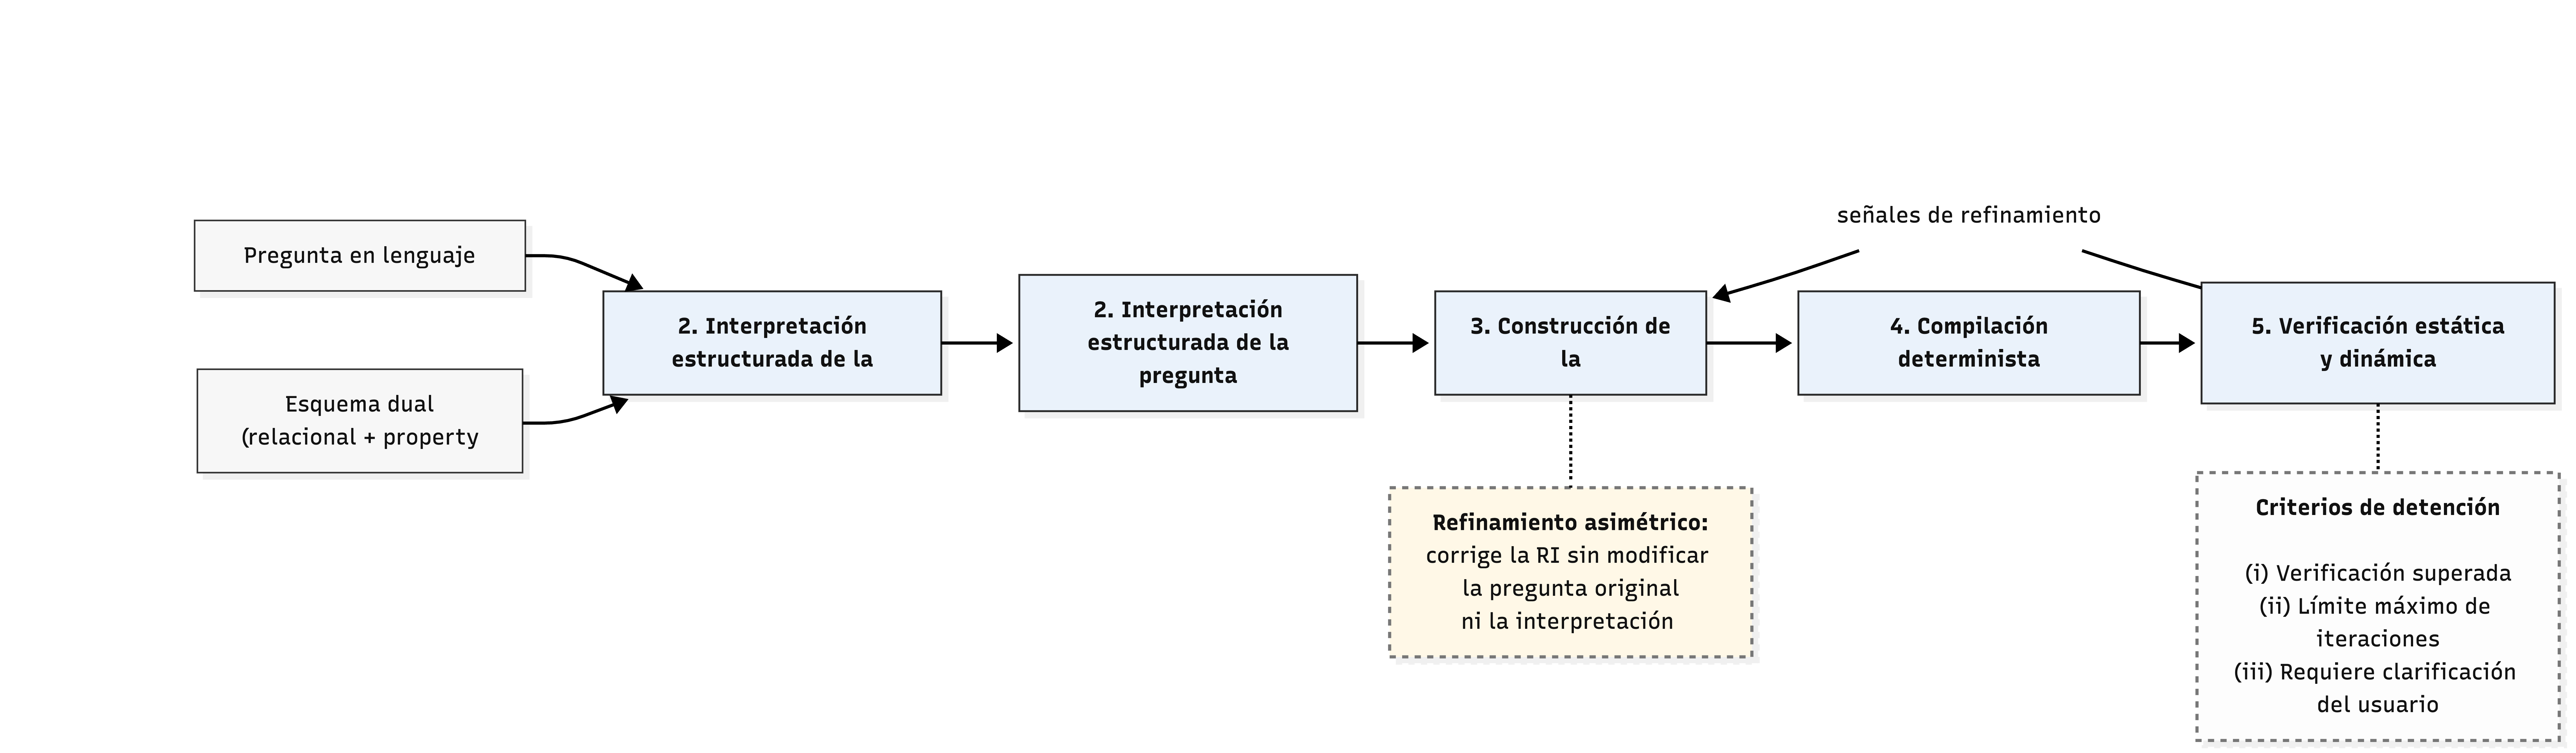
\includegraphics[width=\linewidth]{figs/Chap4/pipeline-general.png}
    \caption{Flujo metodológico general del \emph{pipeline} propuesto. Las
    cinco etapas secuenciales procesan la pregunta en lenguaje natural y el
    esquema dual (relacional y grafo de propiedad) hasta producir una
    consulta \ac{SQL}/\ac{PGQ} verificada.}
    \label{fig:pipeline-general}
\end{figure}

\begin{enumerate}
    \item \textbf{Pre-procesamiento y anclaje al esquema dual.} Esta etapa
    recibe como entrada la pregunta en lenguaje natural, el esquema
    relacional y la definición del grafo de propiedad. Su salida es un
    esquema proyectado, es decir, un subconjunto del esquema dual enriquecido
    con señales de relevancia, tales como tablas y columnas candidatas,
    vértices y aristas potencialmente implicados, así como \emph{cell-values}
    relevantes. Esta fase materializa el principio P1 y se apoya en ideas de
    anclaje al esquema y reducción del espacio de búsqueda reportadas en
    \cite{RSL-SQL2024, CHESS2024}.

    \item \textbf{Interpretación estructurada de la pregunta.} A partir de la
    pregunta y del esquema proyectado, esta etapa produce una descomposición
    explícita de la intención del usuario en componentes interpretables:
    entidades mencionadas, restricciones, proyecciones esperadas y tipo de
    razonamiento requerido. En particular, identifica si la consulta demanda
    razonamiento relacional, razonamiento sobre grafos o una combinación de
    ambos. Esta etapa se inspira en el paradigma de descomposición presentado
    en \cite{DIN-SQL2023, MAC-SQL2023}, extendiéndolo al contexto híbrido
    \ac{SQL}/\ac{PGQ}.

    \item \textbf{Construcción de la representación intermedia tipada.} Con
    base en la interpretación estructurada, se construye una instancia de la
    \ac{RI} propuesta. Esta etapa constituye el núcleo conceptual de la
    arquitectura, pues traduce la intención del usuario a una forma
    estructurada, tipada y validable antes de cualquier compilación al
    lenguaje de consulta final.

    \item \textbf{Compilación determinista a \ac{SQL}/\ac{PGQ}.} Una vez que
    la \ac{RI} satisface sus restricciones estructurales, se compila a una
    consulta concreta mediante reglas deterministas, sin intervención
    adicional del \ac{LLM}. De este modo, la generación estadística queda
    separada de la síntesis sintáctica final, y la consulta producida se
    ajusta por construcción a la gramática del estándar objetivo.

    \item \textbf{Verificación estática y dinámica.} La consulta compilada se
    somete, en primer lugar, a una verificación estática orientada a comprobar
    su consistencia estructural respecto del esquema dual. Si supera esta
    fase, se procede a una verificación dinámica mediante ejecución controlada
    sobre DuckPGQ~\cite{DuckPGQ}. Los errores detectados en cualquiera de
    estos dos niveles se transforman en señales de refinamiento que
    retroalimentan la etapa de construcción de la \ac{RI}.
\end{enumerate}

El bucle de refinamiento es asimétrico en el sentido que la
retroalimentación no modifica la pregunta original ni reabre la interpretación
de alto nivel de la etapa dos, sino que actúa exclusivamente sobre la
construcción de la \ac{RI}. Esta decisión responde al principio P2, ya que
concentra la corrección en el espacio donde la estructura puede manipularse de
forma explícita y verificable mediante reglas. El refinamiento concluye cuando
se satisface alguno de los siguientes criterios: (i) la verificación es
superada, (ii) se alcanza un número máximo de iteraciones, o (iii) el sistema
determina que la pregunta presenta una ambigüedad intrínseca que requiere
clarificación del usuario, en consonancia con lo planteado por
\cite{AmbiSQL}.






\section{Arquitectura y componentes}
\label{sec:prop-arquitectura}

\section{Implementación sobre la base experimental}
\label{sec:prop-implementacion}

\section{Justificación de decisiones de diseño}
\label{sec:prop-justificacion}

\section{Síntesis y transición}
\label{sec:prop-sintesis}
 %Inserta el capítulo 4
\chapter{Experimentos}\label{chap:experiments}
 %Inserta el capítulo 4
\chapter{Resultados}\label{chap:results} %Inserta el capítulo 4
\input{conclusiones} %Inserta el capítulo 5

%%%%%%%%%%%%%%%%%%%%%%%%%%%%%%%%%%%%%%%%%%%%%%%%%%%%%%%%%%%%%%%%%%%%%%

\bibliographystyle{apalike}

\bibliography{Bibliog}
\addcontentsline{toc}{chapter}{Bibliografía}
\end{document}
